\documentclass{report}
% \renewcommand{\thesection}{\arabic{section}}
\setcounter{tocdepth}{1}
% index
\usepackage{imakeidx}
\makeindex%[title=Index, intoc]
% glossary
% \usepackage{glossaries}
% \makeglossaries
% geometry formatting
\usepackage{authblk}
\usepackage[utf8]{inputenc}
\usepackage[margin=0.75in]{geometry}
\usepackage{parskip, setspace}
\setstretch{1.15}
% math formatting
\usepackage{amsmath, amsfonts, braket}
% \numberwithin{equation}{section}
% rich text
\usepackage{graphicx, caption, subcaption, wrapfig, animate}
\usepackage{hyperref}
\usepackage{xcolor}
\hypersetup{
    colorlinks=true,
    linkcolor=black,  
    urlcolor=blue,
    citecolor=blue,
    pdftitle={A Survey of Computational Physics},
    pdfpagemode=FullScreen,
}
% bibliography
\usepackage{biblatex}
\addbibresource{bib.bib}

% \renewcommand{\arraystretch}{1.5} % give a little more space in table

\title{CS 530: High-Performance Computing \\ Seminar 1: A Survey of Computational Physics}
\author{Nathan Chapman}
\affil{Department of Computer Science \\ Central Washington University}
\date{\today}

\begin{document}

\maketitle

\tableofcontents

% \listoffigures

%     \chapter{Error}

%     \chapter{Lax Equivalence Theorem}

%     \chapter{Courant-Friedrichs-Lewy condition}

%     \chapter{Von Neumann Stability}

%     \chapter{Energy Drift}

%     \chapter{Stiff Differential Equations}

%     \chapter{Grids \& Meshes}

%     \chapter{Numerical Diffusion}

\chapter{Introduction}

    Each of the five pillars of physics (Classical Mechanics\index{Mechanics}\index{Mechanics!Classical}, Electromagnetism\index{Electromagnetism}, Relativity\index{Relativity}, Quantum Mechanics\index{Mechanics!Quantum}, and Thermodynamics\index{Thermodynamics}) has well-posed problems for which the mathematical models are either unreasonable or impossible to solve by hand.  As such, computational methods are needed to get an approximate solution.  
    
    There are many numerical methods to support the evolution of physical models for each domain.  Whether it be using a fourth-order Runge-Kutta\index{Runge-Kutta} method to solve the first-order ordinary differential equation \index{Differential Equation!Ordinary} that models a ballistic object under the influence of gravity and air-resistance, or using an eigth-order symplectic\index{Symplectic} Yoshida integrator\index{Integrator!Symplectic} to model a system of bodies orbiting each other while accounting for the produced gravitational waves, there are methods for every physical context.  Though, because these methods are using approximations to their analytic counterparts in calculus, there is error that needs to be considered.

    Numerical analysis\index{Numerical Analysis} is the practice of tracking and rigorously accounting for the discrepancies that arise when approximating analytic mathematical methods by their finite and counterparts.  These errors can arise not only from approximating descriptions from calculus, but also from operations in linear algebra as they're applied to finding the eigenvalues of quantum operators.

\chapter{Classical Mechanics} \label{sec:classical}

    The ``everyday'' world as we know it is described by a model of physics that has been studied for millenia.  As such, we call this model of the behavior of nature ``Classical Mechanics''\index{Mechanics!Classical}.  Now I hear you ask ``Why?''.  Well ``mechanics''\index{Mechanics} is the study of motion, and we include the ``classical'' preface to distinguish it from ``modern'' physics which encompasses all the physics discovered after around 1905 or 1925 (depending on who you ask); those physics will be covered later in sections \ref{sec:quantum} and \ref{sec:relativity}.  For now we take a look at the mathematical model that describes the motion of not-too-small, not-too-large objects moving at slow velocities.
    
    The motion of ``classical'' objects, ranging in scale from biological cells, sand, ants, birds, cars, airplanes, planets, up to stars, can described as the solution to what's called the \emph{equation of motion}\index{Equation of Motion}.  The equation of motion for an object with mass $m$ under the influence of forces $F_i$ is determined by Newton's 2nd law of motion\index{Newton!2nd Law}
    
    \begin{equation} \label{eq:newton}
        \sum_i \mathbf{F}_i = m \ddot{\mathbf{x}},
    \end{equation}

    where $\ddot{\mathbf{x}}$ represents the second time derivative\index{Derivative} of the position\index{Position} $\mathbf{x}$ known as \emph{acceleration}\index{Acceleration}.  These forces completely determine the how objects move through space in time.
    
    Mathematically, the resulting equation is a vector second-order ordinary differential equation\index{Differential Equation!Second Order}, compactly representing the underlying system of differential equations\index{Differential Equation!System}.  In many cases, this differential equation is homogenous\index{Differential Equation!Homogenous} to represent no time-dependent external forces supplying the physical system with energy\index{Energy}.  Likewise, sometimes these forces can be represented by nonlinear\index{Nonlinear} terms; making the equation of motion much more complex.
    
    The following is a survey of topics in classical mechanics whose forces yield an equation of motion either too complex or too unreasonable to solve by hand.

\pagebreak

    \section{N-Body Orbits} \label{subsec:orbits}

        While so-called N-Body\index{N-Body} problems are prolific in physics and other sciences, a quintessential example is the gravitational\index{Gravity} interaction of astrophysical bodies i.e. massive bodies in space.

        \subsection{Mathematical Model: Systems of Ordinary Differential Equations}

            In the case of multi-body gravitaitonal interactions, the governing equation of motion\index{Equation of Motion} is determined via Newton's law of gravitation\index{Newton!Gravitation} between two objects with masses $m_i$ and $m_j$

            \begin{equation}
                F_{ij} = \frac{G m_i m_j}{r_{ij}^2} \hat{r}
            \end{equation}

            where $G = 6.67 \times 10^{-11} \frac{N m^2}{kg^2}$ is the universal gravitaional constant, $r_{ij}$ is the distance between the two objects, and $\hat{r}$ is the unit vector pointing from object $i$ toward $j$.  Not only are is there an equation of motion for each object, but each equation is coupled to every other equation.  This results in the three-dimensional vector differential equation\index{Differential Equation}\cite{taylor2005classical}

            \begin{equation}
                \sum_{j; i \neq j} \frac{G m_i m_j}{(x_i - x_j)^2 + (y_i - y_j)^2 + (z_i - z_j)^2} \frac{(x_j - x_i) \hat{x} + (y_j - y_i) \hat{y} + (z_j - z_i) \hat{z}}{\sqrt{(x_i - x_j)^2 + (y_i - y_j)^2 + (z_i - z_j)^2}} = m_i (\ddot{x_i} \hat{x} + \ddot{y_i} \hat{y} + \ddot{z_i} \hat{z})
            \end{equation}

            for object $i$, and a similar equation for every other object.  For example, a system of 3 objects interacting only via gravitational forces has the equations of motion 

            \begin{align}
                \frac{G m_2}{((x_1 - x_2)^2 + (y_1 - y_2)^2 + (z_1 - z_2)^2)^{3/2}} 
                \begin{bmatrix}
                    x_2 - x_1 \\
                    y_2 - y_1 \\
                    z_2 - z_1
                \end{bmatrix} + 
                \frac{G m_3}{((x_1 - x_3)^2 + (y_1 - y_3)^2 + (z_1 - z_3)^2)^{3/2}} 
                \begin{bmatrix}
                    x_3 - x_1 \\
                    y_3 - y_1 \\
                    z_3 - z_1
                \end{bmatrix} &= \begin{bmatrix}
                    \ddot{x_1} \\
                    \ddot{y_1} \\ 
                    \ddot{z_1}
                \end{bmatrix} \\
                %
                \frac{G m_1}{((x_2 - x_1)^2 + (y_2 - y_1)^2 + (z_2 - z_1)^2)^{3/2}} 
                \begin{bmatrix}
                    x_1 - x_2 \\
                    y_1 - y_2 \\
                    z_1 - z_2
                \end{bmatrix} + 
                \frac{G m_3}{((x_2 - x_3)^2 + (y_2 - y_3)^2 + (z_2 - z_3)^2)^{3/2}} 
                \begin{bmatrix}
                    x_3 - x_2 \\
                    y_3 - y_2 \\
                    z_3 - z_2
                \end{bmatrix} &= \begin{bmatrix}
                    \ddot{x_2} \\
                    \ddot{y_2} \\ 
                    \ddot{z_2}
                \end{bmatrix} \\
                %
                \frac{G m_1}{((x_3 - x_1)^2 + (y_3 - y_1)^2 + (z_3 - z_1)^2)^{3/2}} 
                \begin{bmatrix}
                    x_1 - x_3 \\
                    y_1 - y_3 \\
                    z_1 - z_3
                \end{bmatrix} + 
                \frac{G m_2}{((x_3 - x_2)^2 + (y_3 - y_2)^2 + (z_3 - z_2)^2)^{3/2}} 
                \begin{bmatrix}
                    x_2 - x_3 \\
                    y_2 - y_3 \\
                    z_2 - z_3
                \end{bmatrix} &= \begin{bmatrix}
                    \ddot{x_3} \\
                    \ddot{y_3} \\ 
                    \ddot{z_3}
                \end{bmatrix}
            \end{align}

            Because this problem is in three dimensions, there are actually 9 differential equations to solve in order to fully model the evolution of the position\index{Position} and velocity\index{Velocity} over time of each object.
\pagebreak
        \subsection{Computational Model}
        
            \subsubsection{Finite Differences}

                Because computers can only store numbers of finite precision, approximations must be used in order to implement these differntial equations in a form that can be understood by the computer.  One such translation is by approximating the analytic derivatives and differential operators with \emph{finite differences}\index{Finite Differences}. In its most basic form, the derivative\index{Derivative} can be approximated as a ratio of differences in the form

                \begin{equation}
                    \frac{df}{dt} \approx \frac{f(t + \Delta t) - f(t)}{\Delta t}.
                \end{equation}

                This equation is known as the first-order-accurate\index{Finite Differences!First Order}, forward-finite-difference\index{Finite Differences!Forward} representation of the first-order derivative\index{Derivative!First Order}.  There are similar representations for higher-order derivatives, more accurate approximations, and more accurate approximations of higher-order derivatives. Similarly, there are also \emph{central}\index{Finite Differences!Central} and \emph{backward}\index{Finite Differences!Backward} finite-differences.

                Each of these finite-difference schemes can be represented via coefficients\index{Finite Differences!Coefficients}.  For example, the derivative of order $m$\index{Derivative!Order} with accuracy $n$\index{Finite Differences!Accuracy} has $2p + 1 = 2 \lfloor \frac{m + 1}{2} \rfloor - 1 + n$ central\index{Finite Differences!Central} coefficients $a_{-p}, a_{-p + 1}, \ldots, a_{p - 1}, a_p$ defined such that

                \begin{equation}
                    \begin{bmatrix}
                        1         & 1             & \ldots & 1            & 1 \\
                        -p        & -p + 1        & \ldots & p - 1        & p \\
                        (-p)^2    & (-p + 1)^2    & \ldots & (p - 1)^2    & p^2 \\
                        \vdots    & \vdots        & \vdots & \vdots       & \vdots \\
                        (-p)^{2p} & (-p + 1)^{2p} & \ldots & (p - 1)^{2p} & p^{2p} 
                    \end{bmatrix}
                    \begin{bmatrix}
                        a_{-p} \\
                        a_{-p + 1} \\
                        \vdots \\
                        \vdots \\
                        a_p
                    \end{bmatrix} = 
                    \begin{bmatrix}
                        0 \\
                        \vdots \\
                        m! \\
                        \vdots \\
                        0
                    \end{bmatrix}
                \end{equation}

                where the only non-zero value on the right side of the equation is at the $m+1$-th index.
                
                Once the derivative\index{Derivative} operators are discretized\index{Discretize} using finite-differences\index{Finite Differences}, there are different algorithms in which the differences are used to solve the differential equations\index{Differential Equation}.

            \subsubsection{Symplectic Integrators}

                While there are many methods of numerically solving differential equations\index{Differential Equation} (known as \emph{integrators}\index{Integrator}), one of the most important classes when considering a context such as orbital mechanics\index{Mechanics} and oscillatory\index{Oscillatory} situations (i.e. Hamiltonian\index{Hamiltonian} systems) is that of \emph{symplectic} integrators\index{Integrator!Symplectic}.  This type of integrator is so important to computational physics because it conserves energy\index{Energy!Conservation} throughout time\index{Time} .  Without energy conservation\index{Energy!Conservation}, the system becomes unphysical, which can lead to unnatural behavior such as a mass\index{Mass} on a spring\index{Spring} extending to infinity.  Two of the simplest symplectic integrators\index{Integrator!Symplectic} are the \emph{Semi-implicit Euler Method}\index{Euler}\index{Implicit}

                \begin{subequations} \label{eq:semiEuler}
                    \begin{equation}
                        v_{n+1} = v_n + a_n \Delta t
                    \end{equation}
                    \begin{equation}
                        x_{n + 1} = x_n + v_{n+1} \Delta t
                    \end{equation}
                \end{subequations}

                and the \emph{Velocity Verlet Algorithm}\index{Velocity}\index{Verlet}

                \begin{subequations} \label{eq:verlet}
                    \begin{equation}
                        v_{n+1} = v_n + \frac{a_n + a_{n+1}}{2} \Delta t
                    \end{equation}
                    \begin{equation}
                        x_{n + 1} = x_n + v_{n} \Delta t + \frac{1}{2} a_n \Delta t^2
                    \end{equation}
                \end{subequations}

            \subsubsection{Parallel Computing}

                Because there are so many terms and equations, and each term is only needs the current step, this problem naturally lends itself to being parallelized\index{Parallel} both over the objects\cite{parallelnbody} and in time\cite{LIONS2001661}.

        \subsection{Numerical Analysis}

            \subsubsection{Discretization}

                Error\index{Error} associated with the size of the time-step\index{Step!Time} is dictated by which specific finite-difference\index{Finite Differences} method is chosen.

            \subsubsection{Energy Drift}

                In the case of orbital mechanics\index{Mechanics}, there is no loss of mechanical energy\index{Energy} (ignoring the effects of general relativity; more on this later in section \ref{sec:relativity}).  Therefore, a constraint is imposed on the system that the total mechanical energy\index{Energy} (kinetic energy + potential energy) of the system must remain constant at each point in time\index{Time}.  When using non-symplectic\index{Integrator!Symplectic} methods, this constraint is not adhered to which leads to \emph{energy drift}\index{Energy!Drift}.

\pagebreak
\chapter{Electromagnetism}

    In a general setting, modelling how the electric and magnetic fields change in time and space requires the solutions to \emph{Maxwell's Equations}\index{Maxwell's Equations}\cite{griffiths2017introduction}, succinctly represented as

    \begin{equation}
    \begin{aligned}
        \nabla \cdot \mathbf{E}  &= \frac{\rho}{\epsilon_0}                 & \nabla \cdot \mathbf{B}  &= 0 \\
        \nabla \times \mathbf{E} &= -\frac{\partial \mathbf{B}}{\partial t} & \nabla \times \mathbf{B} &= \mu_0 \mathbf{J} + \mu_0 \epsilon_0 \frac{\partial \mathbf{E}}{\partial t}.
    \end{aligned}
    \end{equation}

    Expanded, these equations take the form

    \begin{equation}
    \begin{aligned}
        \partial_x E_x(t, \mathbf{r}) + \partial_y E_y(t, \mathbf{r}) + \partial_z E_z(t, \mathbf{r}) &= \frac{\rho}{\epsilon_0}                 & \partial_x B_x(t, \mathbf{r}) + \partial_y B_y(t, \mathbf{r}) + \partial_z B_z(t, \mathbf{r})  &= 0 \\
        \begin{bmatrix}
            \partial_y E_z - \partial_z E_y \\
            \partial_z E_x - \partial_x E_z \\
            \partial_x E_y - \partial_y E_x \\
        \end{bmatrix} &= -\partial_t \begin{bmatrix} B_x \\ B_y \\ B_z \end{bmatrix} & \begin{bmatrix}
            \partial_y B_z - \partial_z B_y \\
            \partial_z B_x - \partial_x B_z \\
            \partial_x B_y - \partial_y B_x \\
        \end{bmatrix} &= \mu_0 \rho \begin{bmatrix} v_x \\ v_y \\ v_z \end{bmatrix} + \mu_0 \epsilon_0 \partial_t \begin{bmatrix} E_x \\ E_y \\ E_z \end{bmatrix}.
    \end{aligned}
    \end{equation}

    In their expanded form, Maxwell's equations form a coupled\index{Differential Equation!Coupled} system\index{Differential Equation!System} of eight \emph{partial} differential equations\index{Differential Equations!Partial} (i.e. differential equations whose solutions depend on more than one variable).  Because each of these equations must be solved simultaneously, modelling the dynamics of the electromagnetic field throughout space is quite challenging.  In general solving these equations as presented would require high-performacne computing, but there are simpler cases where such care is not needed.

\pagebreak

    \section{Fringing Electric Fields of Non-Ideal Capacitors}

            The following is taken from previous work\cite{fringingfieldsBealeChapman2019} completed in my undergraduate course in computational physics.

        \subsection{Mathematical Model}

            The behavior of the electric field strength in a parallel plate capacitor can be well understood simply using the classical electromagnetism equation $E = \Delta V / d$ where $V$ is the potential difference between the two parallel plates of the capacitor and $d$ is the distance between them. However, this assumes the plates are infinitely large and ``close'' together.  A consequence of this assumption is a constant electric field between the plates and far from the edge in the finite case. We will be exploring the \emph{fringing field}, or the field that exists outside the area between the capacitors and close to the edges.

            While the fringing field is extremely difficult to model analytically, we can make use of the fact that the electric field is proportional to the gradient of the electric potential.  Since the electric potential is smooth, we can consider the electric potential at any point being the average of the electric potential of it's surrounding points. This is a simplified explanation, but as it turns out we can use this idea to model the potential field numerically.

        \subsection{Computational Model}

            We model the electric potential of a parallel plate capacitor in a grounded box with the \emph{relaxation method} and via the \emph{Gauss-Seidel} (GS) implementation
        
            \begin{equation} \label{eq:GS}
                V_{new}[i,j]=\frac{1}{4}(V_{old}[i+1,j] +V_{new}[i-1,j]+V_{old}[i,j+1]+V_{new}).
            \end{equation}
            
            To strive for maximum computational efficiency, we augment the GS method with a \emph{Simultaneous Over-Relaxation} (SOR) as well. Our SOR method is implemented by augmenting the new potential as 
            
            \begin{equation} \label{eq:SOR}
                V_{new}[i,j]=\alpha \Delta V +V_{old}[i,j],
            \end{equation}
            
            where $\alpha$ is the relaxation coefficient defined by $\alpha = 2 / (1+ \pi / L)$, and $\Delta V$ is the difference between the new value of the potential and the old one.  With the inclusion of SOR, our computation time decreases by a factor of $L$ when compared to not including SOR.  Though, since this implementation is done numerically, several parameters of the system must be stipulated beforehand.
            
            First we will model our parallel plate capacitors to have a potential difference of $2 V$ (our left capacitor will be $1 V$ and our right will be $-1 V$), and we will place it in a grounded box of length $L$.  The size of the box, or correspondingly the size of the capacitor, are natural length scales for the problem and one can be defined in terms of the other.
            
            As a preliminary step in simulating the system numerically, we must discretize our region into cells of side length $\Delta x$.  To make sure our simulation is at least somewhat accurate, $\Delta x$ should be significantly smaller than the total side length of the grounded/bounding box. This will allow us to assign values of the electric potential to actual areas in the box.  This reassignment, from initial ``best guess'', takes the form of the GS method, shown in Equation \ref{eq:GS}.

            Now that we have a method to determine the potential of a point based on surrounding points, we will need to apply it to our model of the physical system. We will need each 'cell' to have an initial value to use our method, and so we will make an 'initial guess' for all cells that are not part of the boundary conditions. In our case we used an initial guess of $0$ for every point except the capacitors. 
            
            To find a reasonable value for the potential at each point we will need to define convergence criteria to compare against in each iteration of the averaging loop.  This is necessary because after the first round of averaging only the cells bordering the capacitors will have any change at all. The more averages we do, the more cells begin being affected by this relaxation method. Once the outermost cells are being affected, the cells closest to the capacitors have gone through many iterations of the average, and so they are more close to the true value than the outer cells. Therefore we defined convergence criteria, forcing our code to continue running through the averages and recalculating the potential until the $\Delta V$, or the difference in the potential value before and after going through the most recent round of averaging, is less than our convergence criteria, which we set to $10^{-5}$. As the cells closer to the capacitors will reach a point of small $\Delta V$ before outer cells will, we have defined our program such that it will continue running until our \textit{maximum} $\Delta V$ is less than our convergence criteria.
            
            Now that we have a complete distribution of the electric potential in our system, we can take the negative gradient of the potential to find the electric field at each point.  Though, since we're working in a discrete space, we need to rethink about how we take derivatives.

            \begin{figure}[t]
                \centering
                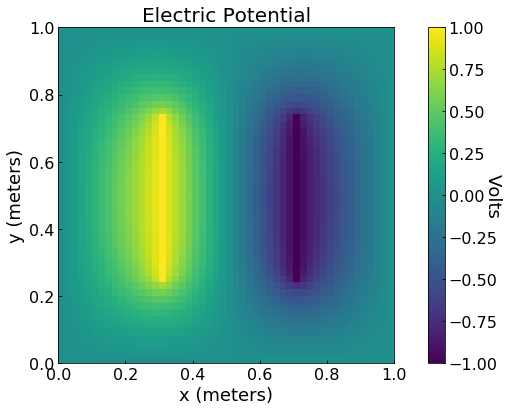
\includegraphics[width=0.45\textwidth]{images/PotentialField.png}
                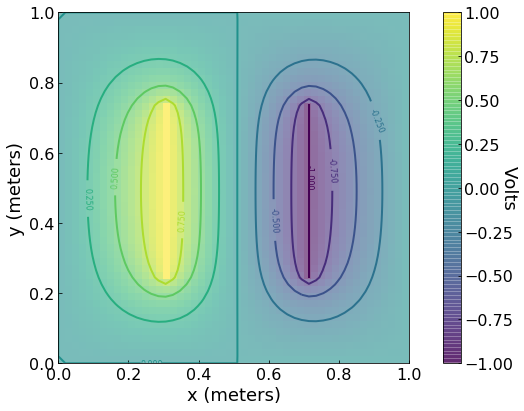
\includegraphics[width=0.45\textwidth]{images/PotentialFieldEquipotentials.png}
                \caption{The electric potential caused by capacitor, whose plates are held at a potential difference of $V=2$, with a boundary condition of $V=0$ at the edges of the box. The left plot shows only the color mapping of the potential while the bottom superimposes equipotential lines separated by $0.25 V$ each on top of the color mapping. The initial guess used for the unknown areas was $0 V$ and the convergence criteria was $10^{-5}$. The box/system is $1 \mathrm{m} \times 1 \mathrm{m}$, while the cell size is $\frac{1}{50^2} \ \mathrm{m^2}$. The separation of the capacitors is 0.4 m and it's length is 0.5 m.}
                \label{fig:PotentialField}
            \end{figure}
            
            To calculate the electric field we will consider a change in potential over a distance, which can be done with the equation
            
            \begin{equation} \label{eq:efieldcomponents}
                \begin{split}
                    E_x &=-\frac{1}{2}\left(\frac{V[i+1,j]-V[i-1,j]}{\Delta x}\right) \\
                    E_y &=-\frac{1}{2}\left(\frac{V[i,j+1]-V[i,j-1]}{\Delta x}\right).
                \end{split}
            \end{equation}
            
            These components can be used to not only show the vector field, but also to give the \emph{magnitude} of the electric field at each point.  The magnitude of the electric field at each point is then the norm of the electric field vectors at the respective points.

            Using the computational methods described in Sec. \ref{sec:Theory}, we created a plot of the potential field within our range. In Figure \ref{fig:PotentialField} we are able to observe the potential across our space. As expected our potential is highest at our left capacitor, with a voltage of +1 V, and lowest at our right capacitor, with a voltage of -1 V. Our boundary conditions at the edge also appear to be near/at zero which is to be expected. 
        
            By looking at the second plot in Figure \ref{fig:PotentialField} we can see that the electric field in between the two capacitors should be fairly constant, which is to be expected as that is the point of capacitors. 
            
            Using Equations \ref{eq:efieldcomponents}, we were able to calculate an electric field for each cell and plot them in a vector plot, shown in Figure \ref{fig:ElectricField}. The electric field looks much like we would expect it to. As we can see in the bottom plot, the electric field vectors are perpendicular to the equipotential lines, which attests to the physical accuracy of of our model. The electric field behaves like we would expect it would, with the fringing field being weaker than the field between the capacitors. The field between the capacitors is relatively constant, which is what we would hope for. We see that there is the highest magnitude electric field right around the edges of the capacitors, which makes sense as that is where the potential will be changing the fastest from the potential of the capacitor to the ground value of the edges.
            
            \begin{figure}[h]
                \centering
                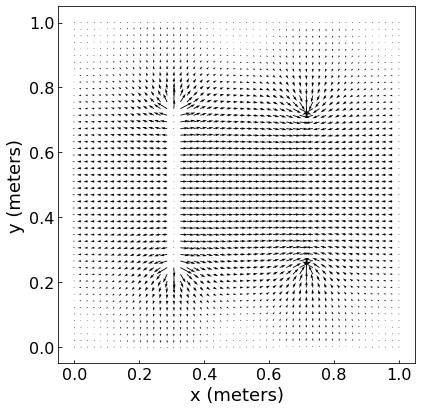
\includegraphics[width=0.27\textwidth]{images/ElectricField.png}
                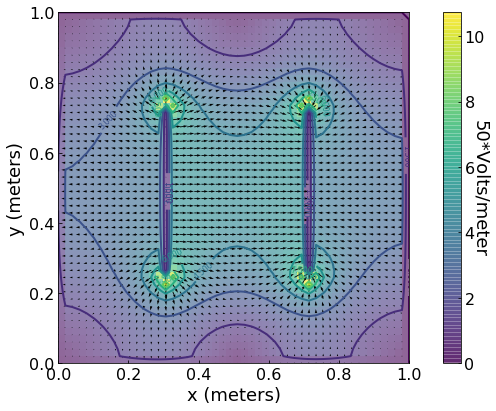
\includegraphics[width=0.32\textwidth]{images/ElectricFieldMagnitude.png}
                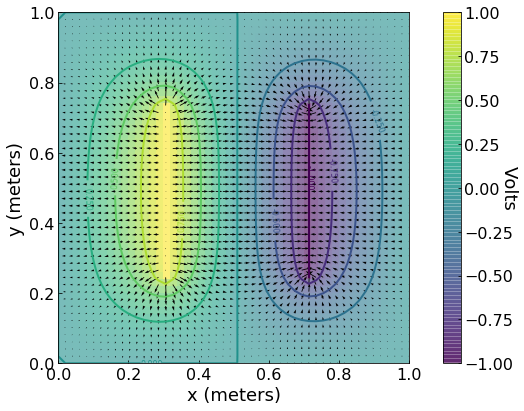
\includegraphics[width=0.34\textwidth]{images/ElectricFieldWithPotential.png}
                \caption{(Left) Electric field in the area of interest. (Center) The top plot shows the electric field vectors on their own, which the second superimposes a color map on top that represents the magnitude of the electric field in $\frac{\text{V}}{\frac{1}{50}\text{m}}$, or 50V/m. The third plot superimposes our potential field on top of the electric field lines. Variables used are the same as in Figure \ref{fig:PotentialField}.}
                \label{fig:ElectricField}
            \end{figure}
            
        \subsection{Numerical Analysis}

            As a final test of the physical accuracy of our model, we chose a spot directly centered between the two capacitors and observed how the electric field at this point changed as the separation of capacitors changed. We did this because for an ideal capacitor we can calculate the electric field simply by using Equation \ref{eq:efield}.
            
            By using both the numerical and analytical solutions shown in Figure \ref{fig:compare} we can conclude that our model seems to be more accurate for smaller seperations and increase in error as the plates get further apart. 
            
            As we can see in Figure \ref{fig:compare}, the error increases as the capacitor separation increases, which makes sense if we look back to how we need more iterations of our Gauss-Streisel SOR method to reach cells that are further away from our boundary conditions. This means that the cell in the center that we are observing has probably only recently met the convergence criteria and so is more prone to error than those that continued to be averaged long past meeting the convergence criteria. 
            
            This also makes sense physically as Equation \ref{eq:efield} assumes a perfect capacitor, which true capacitors will not have perfectly constant electric fields.
            
            As we can explain the error physically and it is small, we can use it as a model for our system.
            
            Finally we observed how cell size affected our results for the electric field. 
            
            The trend shows that as cell size is decreased it trends towards lower percent error in the electric field magnitude and thus towards a numerical convergence. We are not quite sure what the bump near 0.03 cell size means and could not identify a physical or numerical cause. As the rest of the points seems to follow a trend, we chose to make the assumption that the point was inconsistent and do not address it further.

            \begin{figure}[t]
                \centering
                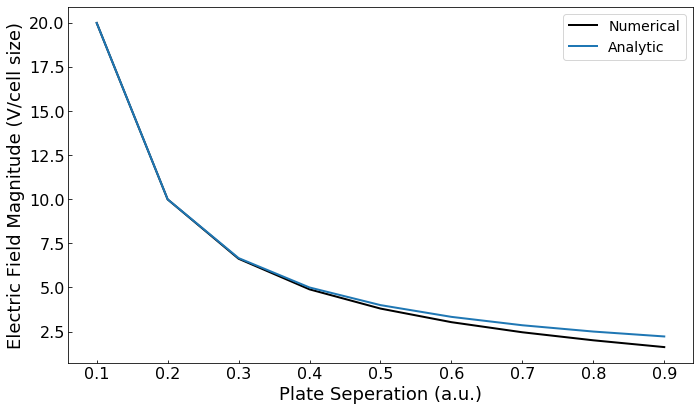
\includegraphics[width=0.48\textwidth]{images/NumericalAnalytic.png}
                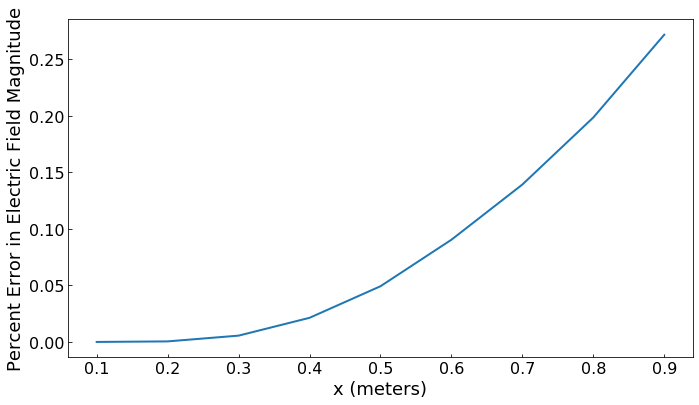
\includegraphics[width=0.49\textwidth]{images/PercentErrorSep.png}
                \caption{The top plot shows the analytic and numerical solution for the electric field magnitude directly between the parallel plate capacitors while the bottom one shows the percent error as a function of plate separation. Other than the varied plate separation, all variables used are the same as used in Figure \ref{fig:PotentialField}.}
                \label{fig:compare}
            \end{figure}
            
            Having confirmed the physical validity of our model, we proceeded to investigate how the fringing field varied with respect to plate separation and distance from capacitor.
        
            As we can see from the plots of the electric field in Figure \ref{fig:ElectricField}, the electric field is strongest at the corners of the capacitor and in between the capacitors and gets weaker as we move further away, into the fringing fields. 
            
            As for the dependence on distance between the capacitors, we were able to plot the electric field for a chosen point outside the capacitors and plot it as a function of changing separation, shown in Figure \ref{fig:sep}.
            
            \begin{figure}[h]
                \centering
                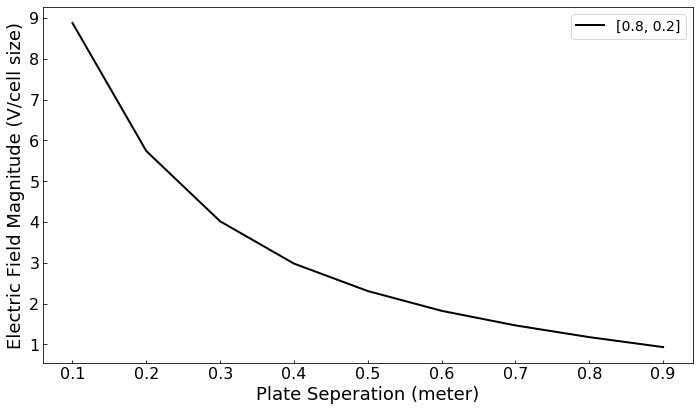
\includegraphics[width=0.66\textwidth]{images/FringeChangingSep.png}
                \caption{The numerically calculated electric field magnitude is plotted above as a function of the separation between the capacitors.}
                \label{fig:sep}
            \end{figure}
            
            In this figure, we can observe that the electric field magnitude at a spot that is 0.5 meters across the cell horizontally and 0.2 meters down from the top ground boundary condition decreases as the plate separation increases.
        
            Our model for the fringing electric field around a capacitor has created a system that seems physically reliable, as shown through it's similarity to the numerical solution in Figure \ref{fig:compare} and when evaluating cell size. Our model has allowed us to observe the fringing field for varying separations and distances from the capacitor. 
            
            Our model is limited in the resolution to which we can model the system, i.e. how small the cell size can be, due to computational time. We used a cell size of 1/50 m for all of our plots except when we were varying cell size and this achieved a resolution that was relatively smooth and resulted in enough data points to evaluate it's accuracy, as shown in Figure \ref{fig:compare}. If we made the cell size smaller, we would get smoother plots of the electric field magnitude and could model the relation to changing variables a bit more accurately, but as we had to calculate so many points for each plot the computation time took significantly longer than the added resolution was worth.
            
            Finally, we saw a weird 'bump' in our plot of the percent error in Figure \ref{fig:cellsize} which interrupted what seemed to be a fairly smooth trend. We were unable to identify the cause of the bump, but as it was small and seemed to still trend towards lower values overall, we are comfortable saying that the percent error in the electric field magnitude decreases with decreasing cell size.

            \begin{figure}[h]
                \centering
                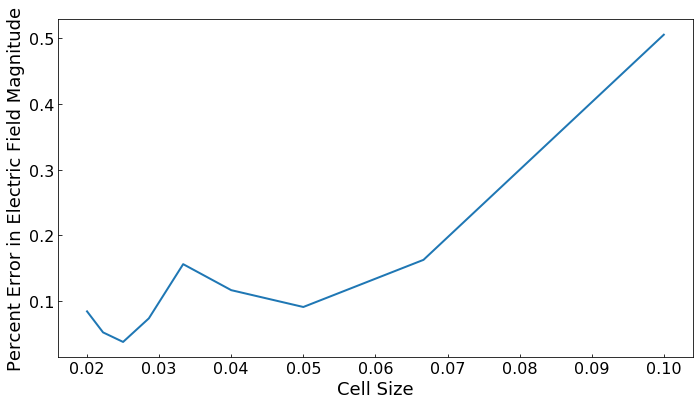
\includegraphics[width=0.66\textwidth]{images/PercentErrorCell.png}
                \caption{The percent error in the Electric Field when using the cell size of 0.01 m as a baseline. Other than varying cell size, all variables used are the same as in Figure \ref{fig:PotentialField}.}
                \label{fig:cellsize}
            \end{figure}

\pagebreak

\chapter{Quantum Mechanics} \label{sec:quantum}

    \section{Quantum Chemistry - Caffeine in Stomach Acid}

        The following is work I completed for the final project in my graduate course ``Chemistry 581: Computational Quantum Chemistry''\cite{Chapman2023}.

        \subsection{Mathematical Model}

            At the heart of quantum mechanics lies the (time-independent) \emph{Schr{\"o}dinger Equation}\index{Schr{\"o}dinger!Equation}

            \begin{equation}
                H \psi = E \psi
            \end{equation}

            where $H$ is a Hermitian operator (i.e. matrix in a basis which is its own conjugate-transpose) known as the \emph{Hamiltonian}\index{Hamiltonian} and $E$ is the (scalar) energy.  Much like how Newton's 2nd Law\index{Newton!2nd Law} determines the motion of classical matter, Schr{\"o}dinger's equation describes the motion of quantum matter.  Thus, the Schr{\"o}dinger equation is the equation of motion in quantum mechanics.
            
            The hamiltonian for a collection of molecules and/or atoms can be represented as\cite{cramer2013essentials}

            \begin{equation}
                H = -\underbrace{\sum_i \frac{\hbar}{2 m_e} \nabla_i^2}_{\text{e motion}} - \underbrace{\sum_k \frac{\hbar}{2 m_e} \nabla_k^2}_{\text{Z motion}} - \underbrace{\sum_{i,k} \frac{e^2 Z_k}{r_{ik}}}_{\text{e-Z interaction}} + \underbrace{\sum_{i < k} \frac{e^2}{r_{ik}}}_{\text{e-e interaction}} + \underbrace{\sum_{k < l} \frac{e^2 Z_k Z_l}{r_{kl}}}_{\text{Z-Z interaction}}
            \end{equation}

            where $\hbar, m_e, e$ are physical constants, $Z$ is an atomic number, $r$ is the distance between two objects, and $i,j$ run over electrons, $k,l$ run over nuclei.  Additionally, recall that $\nabla^2$ is the Laplacian differential operator defined as $\nabla_i^2 = \partial_{x_i}^2 + \partial_{y_i}^2 + \partial_{z_i}^2$, and $r_{ij} = \sqrt{(x_i - x_j)^2 + (y_i - y_j)^2 + (z_i - z_j)^2}$.

            While there are ``mathematically motivated'' methods (e.g. Runge-Kutta) of numerically solving a second-order (linear!) partial differential equation in $3N$ dimensions ($3N$ because each of the $N$ particles has kinetic and interaction energies in 3 dimensions), because of the physical context of the Schr{\"o}dinger equation, another method can be used: Hartree-Fock Self-Consistent Field Theory (SCF).

            The \emph{variational principle}\index{Variational Principle} of quantum mechanics \textit{effectivley} states that for a ``trial'' wave function $\psi^\prime$, the associated energy as given from the Schr{\"o}dinger equation $E$ satisfies $E \geq E_0$, where $E_0$ is the energy of the ``true'' solution $\psi_0$.  Additionally, the trial wave function $\psi$ can be represented as a linear combination $\psi = \sum_i c_i \phi_i$ of orthonormal (i.e. vectors that are orthogonal and have unit magnitude) functions $\phi_i$ from a \emph{basis set}\index{Basis Set}\footnote{3-21G is a simple choice due to its balance between accuracy and speed\cite{cramer2013essentials}.}.  Physically, these basis functions represent single-electron molecular orbitals.  The combination of the variational principle and the ability to represent the trial wave funciton as a linear combination with unknown weights of known functions, transforms the problem of finding the solution to a partial differential equation in $3N$ dimensions into a \emph{minimization problem}\index{Minimization}.

            An example to highlight computational quantum chemistry, because there are many interacting electrons, is in considering the optimal configuration of a caffeine molecule in hydrochloric acid.

        \subsection{Computational Model}

            The Hartree-Fock self-consistent field method (outlined in figure \ref{fig:HFSCF}) (HF SCF) is a way of iteratively solving the many-electron Schr{\"o}dinger equation $H \ket{\psi} = E \ket{\psi}$ for the molecular wave function $\ket{\psi}$.  This is done by replacing the scalar operator $\hat{U}_{ee} = \sum_{i < k} \frac{e^2}{r_{ik}}$ representing the electron-electron repulsion energy by its expectation value $\braket{\hat{U}_{ee}} = \braket{\psi_0 | \hat{U}_{ee} | \psi_0}$, where $\ket{\psi_0}$ is an initial guess e.g. a Gaussian.  The solution $\ket{\psi_1}$ of that Schr{\"o}dinger equation is then used to repeat the process, yielding a (assumingly) more accurate solution $\ket{\psi_2}$.  This nesting process continues until some convergence threshold is met, such as the energy of system doesn't change by more than some amount.

            Considering a single molecule of caffeine (as shown in figure \ref{fig:caffeine}) in the presence of a single HCl molecule while using water as a solvent, the Schr{\"o}dinger equation can be solved to optimize the configuration of each of these molecules using the computational quantum chemistry softwrae \textit{Gaussian}.  Using Density Functional Theory\index{Density Functional Theory} (a highly accurate method in which to implement the SCF), the system can be optimized to the configuration shown in figure \ref{fig:Optimized}.  

            Furthermore, the highest and lowest occupied molecular orbitals can be seen in figure \ref{fig:frontierOrbitals}.

            Finally, the vibrational modes corresponding to the two tallest peaks in the IR spectrum (figure \ref{fig:spectrum}) of the optimal configuration are show in the animated (depending on the pdf viewer used) figure \ref{fig:vibModes}.

        \subsection{Numerical Analysis}

            Many molecules and other chemical systems are well documented on PubChem, including their DFT-optimized configuration.  Comparisons between the unoptimized and optimized systems are shown in figures \ref{fig:PubChem_Energy_APE} and \ref{fig:Method_APE}.

            \begin{figure}[h!]
                \centering
                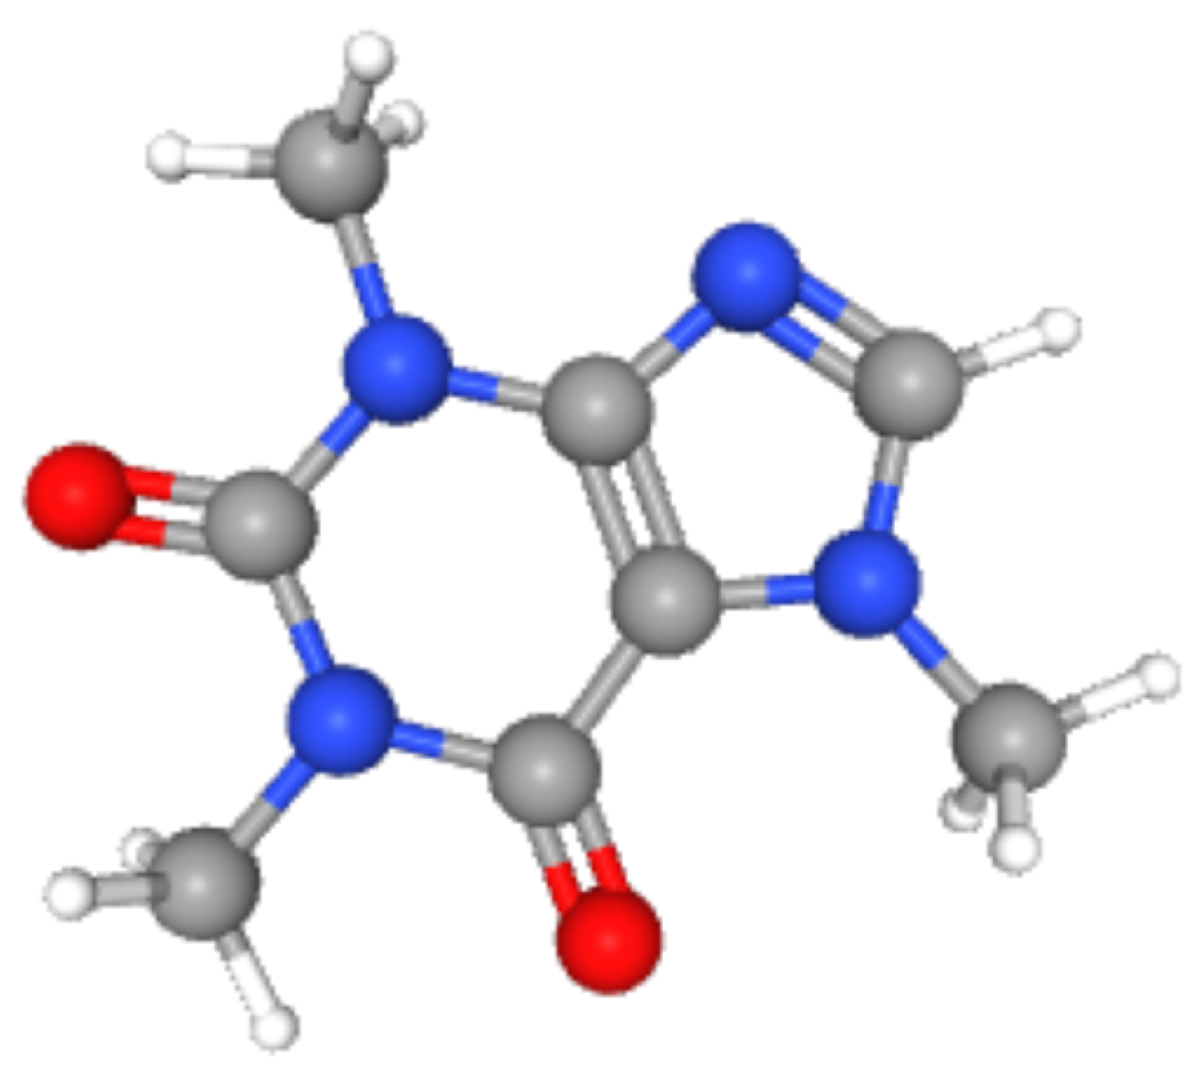
\includegraphics[width=0.5\textwidth]{images/Caffeine.png}
                \caption{A caffeine molecule in its optimal configuration}
                \label{fig:caffeine}
            \end{figure}

            \begin{figure}[h]
                \centering
                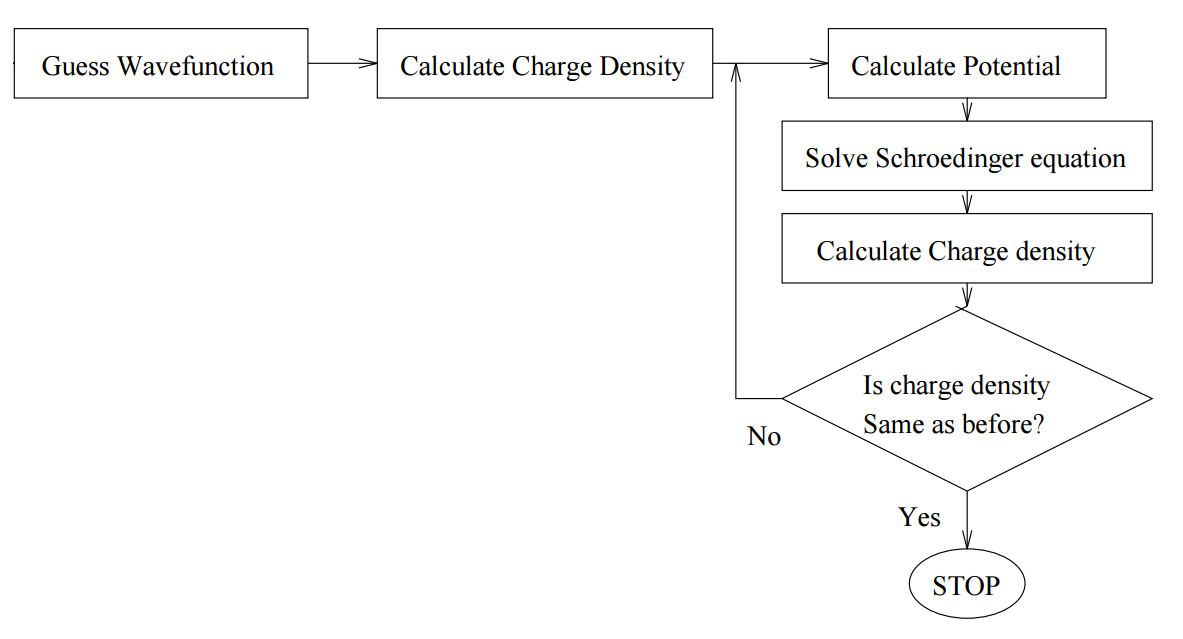
\includegraphics[width = 0.66\textwidth]{images/hartree_fock.png}
                \caption{Diagram\cite{scf} showing the iterative nature of the Hartree-Fock Self Consistent Field Method.}
                \label{fig:HFSCF}
            \end{figure}

            \begin{figure}[h]
                \centering
                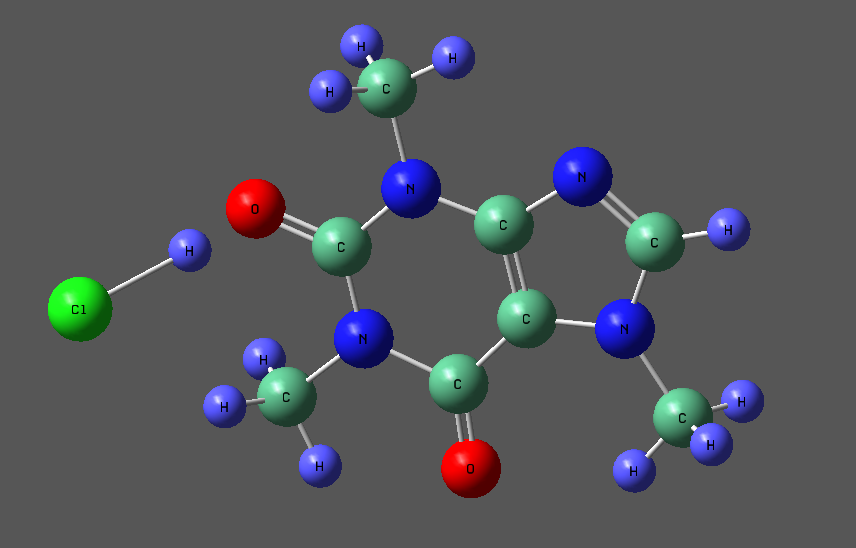
\includegraphics[width=0.67\textwidth]{images/Optimized_Caffeine_HCl.png}
                \caption{DFT optimized caffeine and HCl in water}
                \label{fig:Optimized}
            \end{figure}

            \begin{figure}[h]
                \centering
                \begin{subfigure}[b]{0.45\textwidth}
                    \centering
                    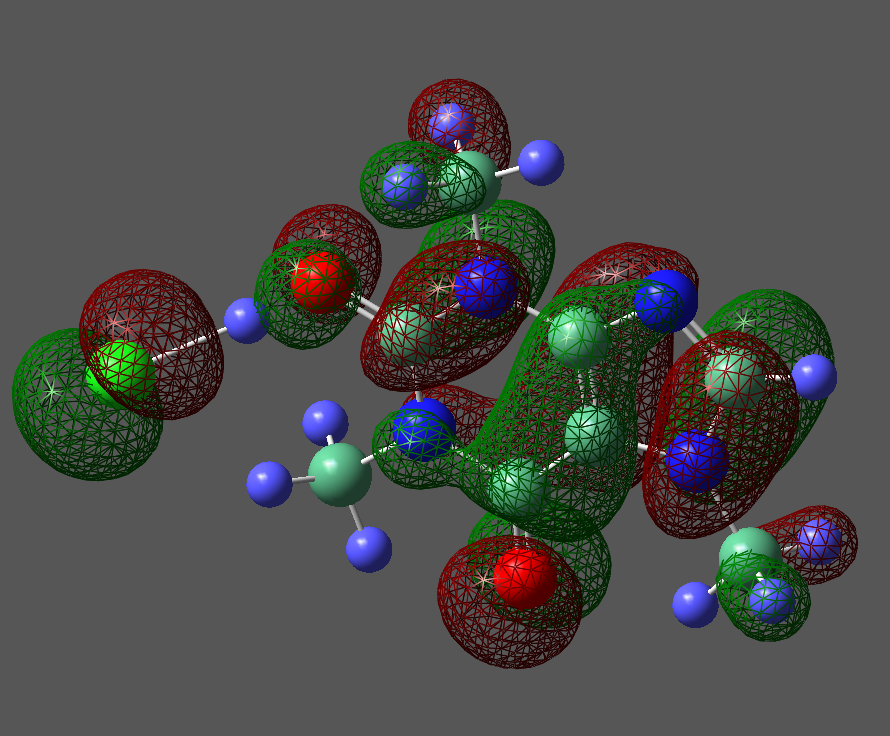
\includegraphics[width=\textwidth]{images/HOMO.png}
                    \caption{Highest Occupied Molecular Orbital}
                    \label{fig:HOMO}
                \end{subfigure}
                \hfill
                \begin{subfigure}[b]{0.45\textwidth}
                    \centering
                    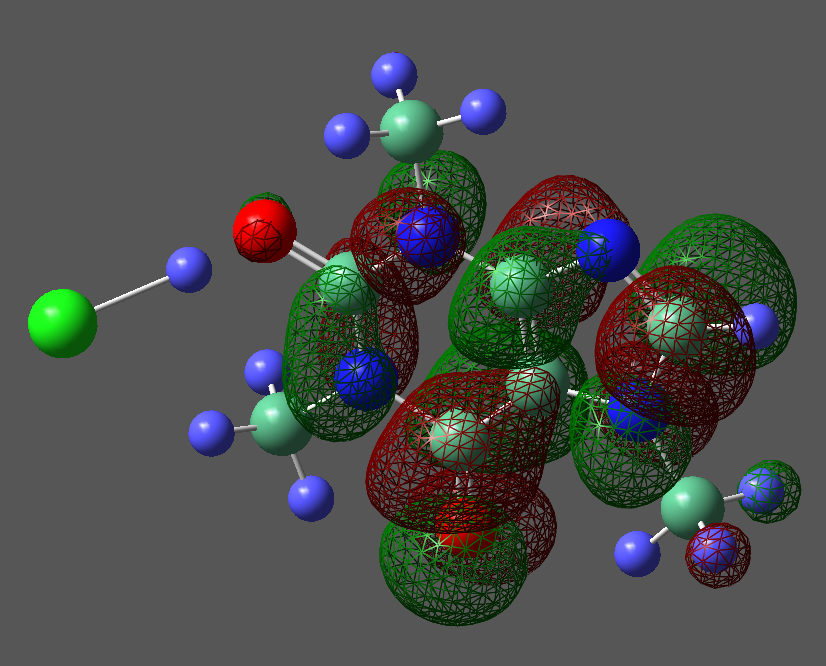
\includegraphics[width=\textwidth]{images/LUMO.png}
                    \caption{Lowest Occupied Molecular Orbital}
                    \label{fig:LUMO}
                \end{subfigure}
                \caption{Frontier molecular orbitals}
                \label{fig:frontierOrbitals}
            \end{figure}

            \begin{figure}[h]
                \centering
                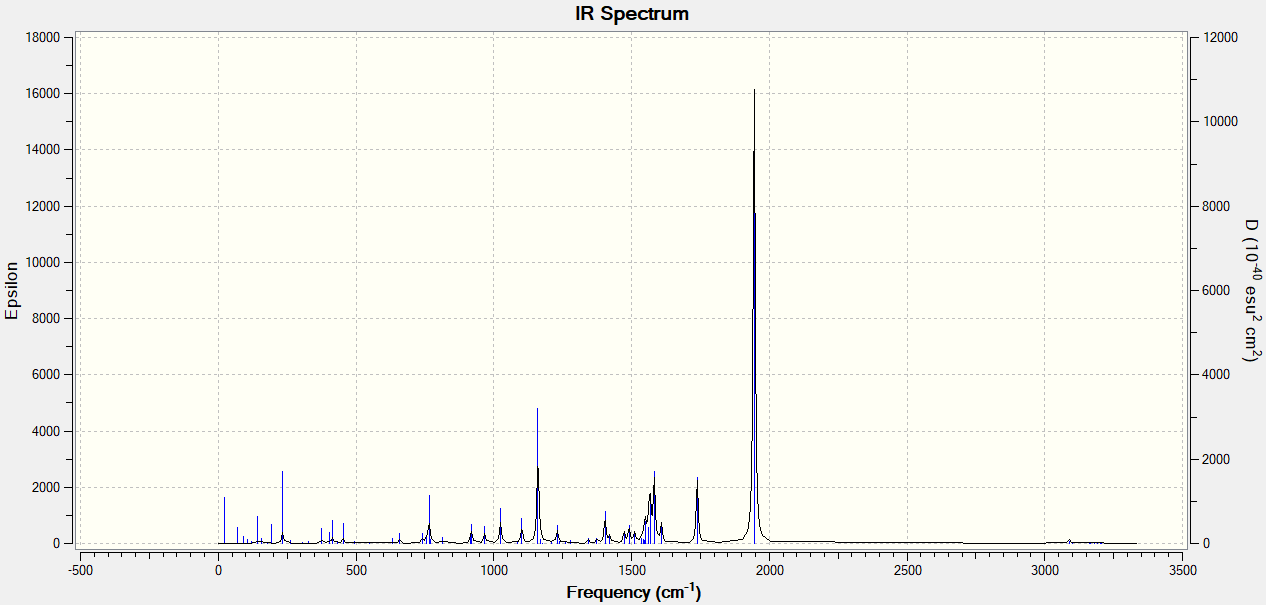
\includegraphics[width=0.67\textwidth]{images/spectrum.png}
                \caption{IR spectrum}
                \label{fig:spectrum}
            \end{figure}

            \begin{figure}[h]
                \centering
                \begin{subfigure}[b]{0.45\textwidth}
                    \centering
                    \animategraphics[loop,controls,width=\textwidth]{20}{images/Low_peak/Low_Peak_}{0000}{0063}
                    \caption{Vibrational mode corresponding to the second tallest peak in the IR spectrum above}
                    \label{fig:LowPeak}
                \end{subfigure}
                \hfill
                \begin{subfigure}[b]{0.45\textwidth}
                    \centering
                    \animategraphics[loop,controls,width=\textwidth]{20}{images/High_peak/peak_1}{0000}{0063}
                    \caption{Vibrational mode corresponding to the tallest peak in the IR spectrum above}
                    \label{fig:HighPeak}
                \end{subfigure}
                \caption{Vibrational modes of the two largest peaks in the IR spectrum}
                \label{fig:vibModes}
            \end{figure}

            \begin{figure}[h]
                \centering
                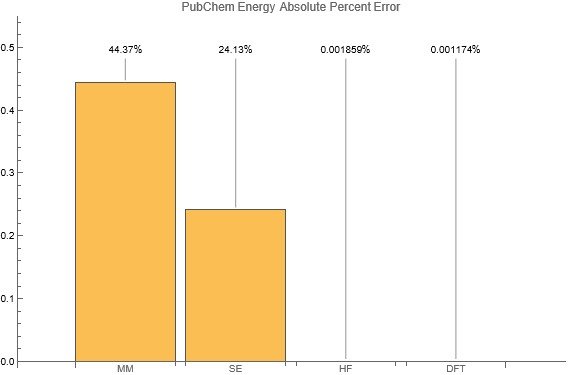
\includegraphics[width=0.67\textwidth]{images/PubChem_Energy_APE.png}
                \caption{Absolute percent error in energy for different methods for the caffeine molecule as given by PubChem}
                \label{fig:PubChem_Energy_APE}
            \end{figure}

            \begin{figure}[h]
                \centering
                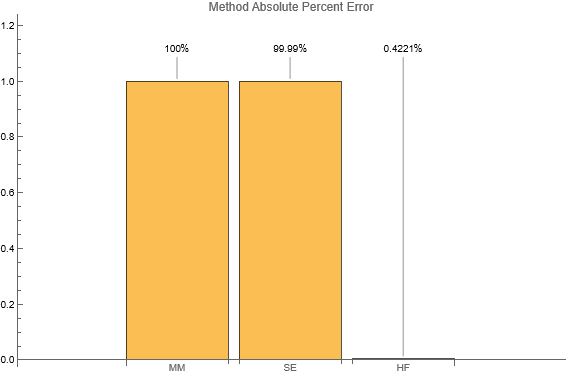
\includegraphics[width=0.67\textwidth]{images/Method_APE.png}
                \caption{Absolute percent error in energy for different methods compared to DFT}
                \label{fig:Method_APE}
            \end{figure}
\clearpage
\newpage

\chapter{Relativity} \label{sec:relativity}

    One of the most fundamental concepts in analytic geometry is the coordinate system\index{System!Coordinate}.  Coordinate systems are composed of scale, direction, and origin\footnote{More technically, these terms scale $\rightarrow$ algebraic field, direction $\rightarrow$ a set of basis vectors}.  Given two coordinate systems, a position in space can be represented in either system, but there also exists a transformation between the two coordinate systems so that if you know the position in one coordinate system and the transformation between the systems, you can calculate the position in the other coordinate system.  This remains true even if the origin of the coordinate system is moving.  The study of how physical properties are represented and change between these coordinate systems is called \emph{relativity}\index{Relativity}.  
    
    While there is Galilean relativity, which deals with objects whose speed is unbounded, more accurate models of physics have been introduced\cite{einstein1905electrodynamics} with a ``universal speed limit'', bounding the speed at which any object can travel.  This model is called \emph{Special Relativity}\index{Relativity!Special}, and this relatively small change (no pun intended) has drastic consequences when considering objects moving at near this speed limit.  These relativistic effects are highlighted when there are many obejcts to compare\footnote{\href{https://youtu.be/qol-zP9W5J4?si=7ty4vfO9ceFox48e}{OpenRelativity} visualization}\cite{openrelativity}.  While it is possible to describe the physics of objects moving near the universal speed limit using simple mathematical tools, in order to have a unified theory that describes both these effects and those that arise when considering how mass plays a role, more complex mathematical tools need to be considered.  As such, more complex Computational Model are needed to get a definitive picture of physics in space and time.

    A different approach to describing Special Relativity is to consider physics not just happening \textit{in} space and \textit{over} time, but rather on a single backdrop that unifies these concepts called \emph{spacetime}\index{Spacetime}.  When considering relativistic effects on this spacetime backdrop, there is not only a coupling between motion relative to different observers, but also between mass and the spacetime itself.  Special Relativity ignores this mass-spacetime coupling, resulting in a \textit{special} case of \emph{General Relativity}\index{Relativity!General}.  In the presence of an object, spacetime bends and warps in a way proportional to the object's mass and energy.  Mathematically, this warping is represented as the curvature of a manifold as described by Differential Geometry.  In the end, this complex description leads to a system of of coupled, nonlinear, partial differential equations that are most often impossible to solve analytically, so numerical methods must be employed.

    The system of ten coupled, nonlinear, second-order, partial differential equations in four dimensions\cite{443754} as mentioned above is called the \emph{Einstein Field Equations}\index{Einstein Field Equations} (EFEs).  The EFEs are notoriously complicated and and yield very few closed-form solutions\cite{misner2017gravitation}, each only being defined for situations with a high-degree of symmetry.  Numerical methods, such as the ADM formalism\cite{Arnowitt_2008}, have been employed to find approximate solutions to the EFEs defining the field of \emph{Numerical Relativity}\index{Relativity!Numerical}.  The physical scenarios considered, such as binary black hole mergers\cite{blackholemerger} and ray tracing near a black hole\cite{James_2015}, yield forms of the EFEs that must be numerically solved with high-performance computing\cite{li2023solving,Andrade2021,Clough_2015}.

\newpage

    The effects of General Relativity (GR) are \emph{mostly} unobservable within our solar system.  One of the exceptions being the precession of Mercury's perihelion.  Due to Mercury's close proximity to the Sun, and its higher-than-average eccentricity, Mercury's orbit around the sun changes in ways unpredicted by Newtonian gravity.  The reason for this discrepancy is that while Mercury orbits the sun, gravitational waves are released and carry energy away from the pair, causing Mercury's motion to change.  This phenomenon has been explored in two aspects: modelling how the eccentricity of Mercury's orbit affects the precession of its perihelion\cite{Chapman2019}, and analysizing the ``chirp'' that arises from the leading-order frequencies of the emitted gravitaitonal waves when the Sun and Mercury merge\cite{Chapman2022}.

    \section{Effects of Eccentricity on the Precession of Mercury's Perihelion}

        The following is work I completed for the final project in my undergraduate course ``Physics 486: Computational Physics''\cite{Chapman2019}.

        \subsection{Mathematical Model}

            Newtonian gravity is simple enough that it is a center piece of all introductory physics courses.  This placement and difficulty is primarily due to the fact that the only mathematical theory encapsulated in this formalism is basic vectors in a Euclidean space, or rather arrows in our 3D world.  Of course the form of gravity a la Newton is
        
            \begin{equation} \label{eq:Newton}
                \mathbf{g} = -\frac{G m}{r^3} \mathbf{r} = -\frac{G m}{r^2} \hat{r},
            \end{equation}
            
            where of course, $G_N$ is the Newtonian gravitational constant, $m$ is the mass of the \emph{central mass}, or rather the object that is causing the gravity, and $r$ is the magnitude of the separation $\mathbf{r}$ between the central mass and a point in space.  This form works extremely well for everyday situations like objects interacting with the Earth, or \emph{most} planets interacting with the Sun.  It is in the latter case, namely Mercury interacting with the Sun, where we find Newtonian gravity is not suitable to describe objects that are interacting via a stronger gravity.  For such situations we must extend our model to the standard treatment of gravity, General Relativity (GR).
            
            General Relativity is, to put it \emph{absurdly} lightly, a step up in difficulty from Newtonian gravity.  Albert Einstein's famous and elegant theory needs much more difficult mathematical machinery to describe the gravitational interactions between objects.  Without going into too much detail, GR requires the use of a field of math called \emph{Differential Geometry} (DG) which describes geometric properties, like distance, in/on curved spaces/surfaces.  The full general relativistic description of gravity gives the Einstein Field Equations (EFE)\cite{MTW}
            
            \begin{equation} \label{eq:EFE}
                G_{\mu \nu} = \frac{8 \pi G_N}{c^4} T_{\mu \nu}
            \end{equation}
            
            where $G$ is the Einstein tensor that describes how space and time curve, and $T$ is the stress-energy tensor that describes how much energy there is in a region.  There are few analytic solutions to this equation, and therefore few instances of exact descriptions of ``true'' gravity.  Therefore, we must usually resort to approximate numerical solutions in order to model the systems that require the full form of GR.  It turns out, even approximating solutions to the EFE are really hard.  Though, there are situations that lend themselves to being modeled via a mix of Newtonian gravity and GR.
            
            GR is definitely needed and to be fully used in the case of masses strongly interacting via gravitation, e.g. near black holes and neutron stars, but what about when the objects aren't massive enough, or are far enough away that they experience GR effects only slightly?  This is called the \emph{weak field limit} (WFL).  The set of systems that obey Newtonian gravity fall into this regime, but also the ones that behave slightly non-Newtonian-ly.  In the WFL, such systems can be modeled with a combination of Newtonian gravity and GR via corrections to the Newtonian form of gravity (Eq. \ref{eq:Newton}).  This combination of theories takes the form of adding corrections to the Newtonian form of gravity as
            
            \begin{equation} \label{eq:MOND}
                \mathbf{g} = -\frac{c^2}{2} \frac{r_s}{r^2} \left( 1 + 3 \frac{r_L^2}{r^2} \right) \hat{r},
            \end{equation}
            
            where $r_s$ is the Schwarzchild radius of a mass defined by 
            
            \begin{equation} \label{eq:Schwarz}
                r_s = \frac{2 G_N}{c^2} m,
            \end{equation}
            
            where $m$ is the mass of the object, and
            
            \begin{equation}
                r_L^2 = \frac{( \mathbf{r} \times \dot{\mathbf{r}} )^2}{c^2}.
            \end{equation}

            Even though the WFL can be modeled via modified Newtonian dynamics (MOND), Newtonian gravity is still easier to implement and understand.  So the natural question arises, at what point are the GR effects significant enough to invoke, at least, MOND?  In figure (\ref{fig:Newton_GR_Comp}), we can see that there is a small but significant difference between Newtonian gravity and the MOND gravity as the distance between masses approaches zero.  At a certain point though, the difference is indeed negligible, and Newtonian gravity can be used without worry.
        
            \begin{figure}[h]
                \centering
                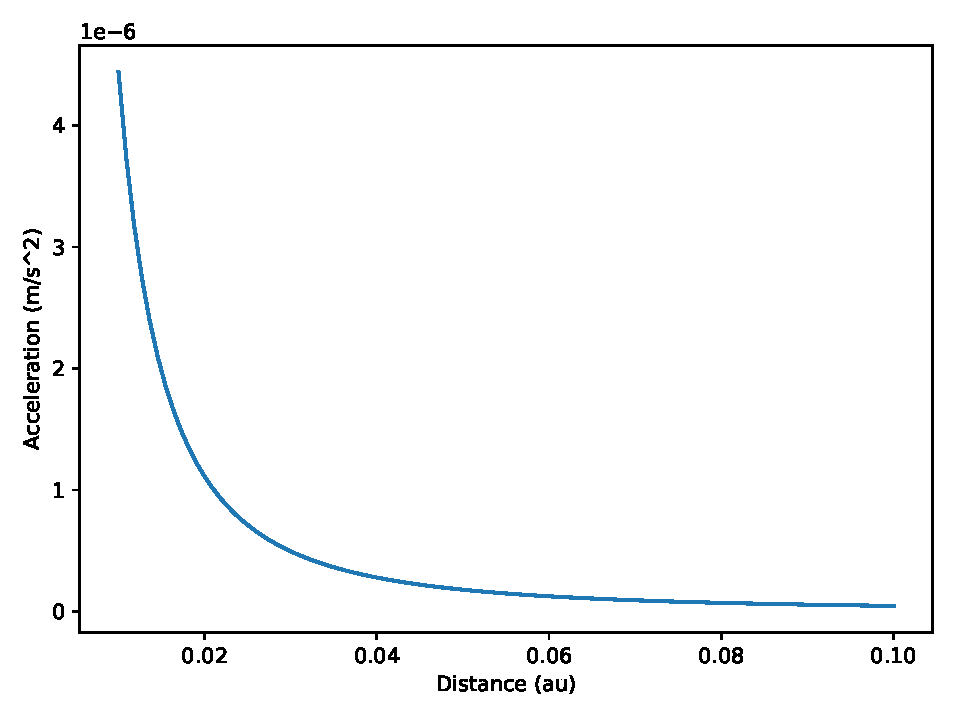
\includegraphics[width = 0.66\textwidth]{images/Newton_GR_Comp.pdf}
                \caption{The absolute difference in gravity between the Newtonian model and the GR model.  The mass used was one solar mass, and the velocity was Mercury's average orbital velocity.}
                \label{fig:Newton_GR_Comp}
            \end{figure}
            
            With this form of gravity, any investigation of a system in the WFL can be carried out as it would with Newtonian gravity.  Though in this work, the precession of periapsides is done computationally, there is an analytic form of the angular precession due to GR.  
            
            GR directly tells us that the radial equation for an orbit is defined as\cite{MTW}
            
            \begin{equation} \label{eq:GR_radius}
                r(\phi) = \frac{(1 - e^2) a}{1 + e \cos[ (1 - \delta \phi_0 / 2 \pi) \phi]}
            \end{equation}

\pagebreak
            
            From equation (\ref{eq:GR_radius}), the angular precession of the orbit is exactly
            
            \begin{equation}
                \delta \phi_0 = \frac{6 \pi M}{a ( 1 - e^2)}
            \end{equation}
            
            where $M$ is mass ``causing'' the gravity, and $a, e$ are the semi-major-axis and eccentricity respectively.

        \subsection{Computational Model}
        
            \textbf{Initialization \& first step:} To start the simulation of these two celestial bodies, one of which is fixed in space at the origin, the program takes as it's initialization parameters the masses of the two orbiting bodies, the initial position of the orbiting body at its periapsis, the initial velocity of the orbiting body at its periapsis, the number of orbits the body will undergo, and whether or not the gravity used will be the modified gravity (Eq. \ref{eq:MOND}) or the standard Newtonian gravity (Eq. \ref{eq:Newton}).  From these parameters, the gravity due to the fixed mass is found at the initial position of the orbiting mass, and the first step in the orbiting mass's orbit is found through an Euler-Cromer method as
            
            \begin{subequations}
                \begin{align}
                    \mathbf{v}_{1} &= \mathbf{v}_0 + \mathbf{g}_0 \Delta t \\
                    \mathbf{r}_{1} &= \mathbf{r}_0 + \mathbf{v}_1 \Delta t
                \end{align}
            \end{subequations}
            
            where $g_0$ is the gravity at the initial position $r_0$ acting on the orbiting mass with velocity $v_0$, and $\Delta t$ is the time step.  We make note of the velocity dependence of gravity here because in Newtonian gravity, the strength of the gravitational acceleration only depends on the distance from the mass, whereas in GR, the strength of gravity is dependant upon the distance and velocity of the mass on which gravity is acting.
            
            \textbf{Time step:} Here we define our time step as above as
            
            \begin{equation} \label{eq:time-step}
                \Delta t = \frac{2 v_0}{\alpha a_0},
            \end{equation}
            
            where $\alpha$ is the factor by which we decrease the time step, and in this work $\alpha = 2000$ (While this seems drastic in the sense that this produces on average a time step of about 15 minutes/sub-hour precision, if any smaller value was chosen, the end results \emph{seemed} completely unphysical).  We choose this time step so the Euler-Cromer evolution of the position is indeed a valid one.  Since the time step is defined as such, it is actually determined by the initial properties of the system, and not in fact a parameter that is given by the user.  After the first step is taken, the model transitions to evolving under a Verlet method.
            
            \textbf{Evolution:} Whereas some models use forward biased methods, like the Euler method \cite{korber2018primer}, here we use the time-reversible Verlet method
            
            \begin{equation} \label{eq:verlet}
                y_{i + 1} = 2 y_i - y_{i - 1} + \left. \frac{d^2 y}{d t^2} \right|_{y_i, t_i} \Delta t^2
            \end{equation}
            
            to ensure energy conservation.  Conservation of energy is of the utmost importance in long-term gravitational simulations because over such long time periods, the error/energy-leak accumulates and makes the end result completely inaccurate.  Now we evolve our system using this time step and integration method.

\pagebreak

            The main evolution of the system is defined by
            
            \begin{subequations} \label{eq:step}
                \begin{align}
                    \mathbf{r}_{i + 1} &= 2 \mathbf{r}_i - \mathbf{r}_{i - 1} + \mathbf{g}(\mathbf{r}_i, \mathbf{v}_i, t_i) \Delta t^2 \\
                    \mathbf{v}_{i + 1} &= \frac{\mathbf{r}_{i + 1} - \mathbf{r}_{i - 1}}{2 \Delta t}
                \end{align}
            \end{subequations}
            
            where the position $\mathbf{r}$ evolves under our Verlet integration, and the velocity $\mathbf{v}$ is determined via a simple difference quotient.  Through this updating algorithm, the system evolves throughout it's orbit for one orbital period.
            
            \textbf{Orbit:}  The system steps through time under (Eq. \ref{eq:step}) for one orbital period.  This orbital period $\tau$ is found through the classical Keplerian formula\cite{taylor2005classical}
            
            \begin{equation} \label{eq:period}
                \tau^2 = \frac{4 \pi^2 \mu}{G_N m_1 m_2} a^3
            \end{equation}
            
            where $G_N$ is the Newtonian gravitational constant, $m_1, m_2$ are the masses of the objects, $\mu = \frac{m_1 m_2}{m_1 + m_2}$ is the reduced mass of the system, and $a$ is the semi-major-axis (SMA).  Here the SMA is defined in terms of other parameters of the system as
            
            \begin{equation} \label{eq:sma}
                a = \frac{c}{1 - \epsilon^2}
            \end{equation}
            
            where $c$ is the \emph{principal orbital parameter} defined by 
            
            \begin{equation} \label{eq:pop}
                c = \frac{l^2}{G_N m_1 m_2 \mu},
            \end{equation}
            
            where $l$ is the magnitude of the angular momentum defined by
            
            \begin{equation} \label{eq:angular-momentum}
                l = m_2 ||\mathbf{r}_0 \times \mathbf{v}_0||
            \end{equation}
            
            and $\epsilon$ is the eccentricity of the orbit defined by
            
            \begin{equation} \label{eq:eccentricity}
                \epsilon = \frac{c}{r_0} - 1
            \end{equation}
            
            After one orbit has been simulated, the periapsis of that orbit is found by simply selecting the position that is closest to the fixed body.  Once the location of the periapsis is known, and since we're interested in how the periapsis precesses, the angle of the periapsis is found with respect to the initial position (i.e. the x-axis because we started there) in arcseconds.  We choose to work in units of arcseconds because we know that the perihelion precession of Mercury due to GR is about 43 arcseconds per century and so the average precession angle should be on that scale.
            
            Now that we have an algorithm to evolve the system for one orbital period, we let the system evolve for as many periods as we want, and measure the positions, velocities, periapsides, the angles of the periapsides, and the eccentricities as we go.
            
            After several orbits have been simulated, we preform a linear regression (with numpy's polyfit function) on the angles of the periapsides throughout the orbits to find the average rate of precession of the orbiting body. (All that work for one number!)

        \subsection{Numerical Analysis}

            Of course no computational model is complete without an analysis of the numerical accuracy.  While there is no \emph{easy} analytic solution to this problem, we can test the sub-processes that govern the overall results.
            
            As above, several parameters are not calculated through recursive formulations but rather through their closed form mathematical definitions.  Even though these properties have a closed form definition, computational calculations still carry error.
            
            \begin{table}[h]
                \centering
                \begin{tabular}{|c||c|c|c|c|}
                    \hline
                    & $r_{S, \odot}$ & $g_\oplus$ & $\epsilon_\text{Mercury}$ & $\tau_\text{Mercury}$ \\
                    \hline
                    \hline
                    Predicted  & 2.953 km & 9.807 m/$s^2$ & 0.205 & 88 Earth days \\
                    \hline
                    Calculated & 2.949 km & 9.813 m/$s^2$ & 0.206 & 88.1 Earth days \\
                    \hline
                    Difference & 0.004 km & 0.006 m/$s^2$ & 0.001 & 0.1 Earth days \\
                    \hline
                    \% Difference & 0.16 & 0.06 & 0.49 & 0.11 \\
                    \hline
                \end{tabular}
                \caption{The calculated and measured values of the Schwarzchild radius of the Sun, the gravity at the surface of the Earth, the eccentricity of Mercury, and the orbital period of Mercury, along with their absolute and percent differences (i.e. percent difference $= |\text{predicted} - \text{calculated}| / \text{predicted}$).}
                \label{tab:val_comp}
            \end{table}
            
            In table (\ref{tab:val_comp}) we compare the values calculated here against the either measured or more accurately computed values.  We can see all properties are within 1\% of their ``accurate'' counter-parts.  While we can quite easily quantify the error in these parameters, we can also at least qualitatively describe the error in the evolution of the system as well.
            
            To test the orbital procedure, we test the trajectory of Earth around the Sun because we know it should be mostly circular.  In figure (\ref{fig:Earth_trajectory}), we see how the trajectory of the Earth behaves for different time steps.  The different trajectories in the figure are not actually the time steps exactly, but rather the scaling parameter $\alpha$ as in equation (\ref{eq:time-step}).  In each of these simulations, Earth started at it's average orbital distance (1 AU) on the x-axis, with its average orbital velocity orthogonal to the position ($v = 2 \pi (1 \mathrm{AU}) / (1 \mathrm{year})$).  We can see that even for relatively small scaling factors ($\alpha = 20$ compared to the factor used for the results was $\alpha = 2000$), the trajectory of Earth converges to its known circular orbit.  Another property we can test to get at least a qualitative idea of the error in our procedure is how the rate of precession varies with the length of the simulation.
            
            \begin{figure}[h]
                \centering
                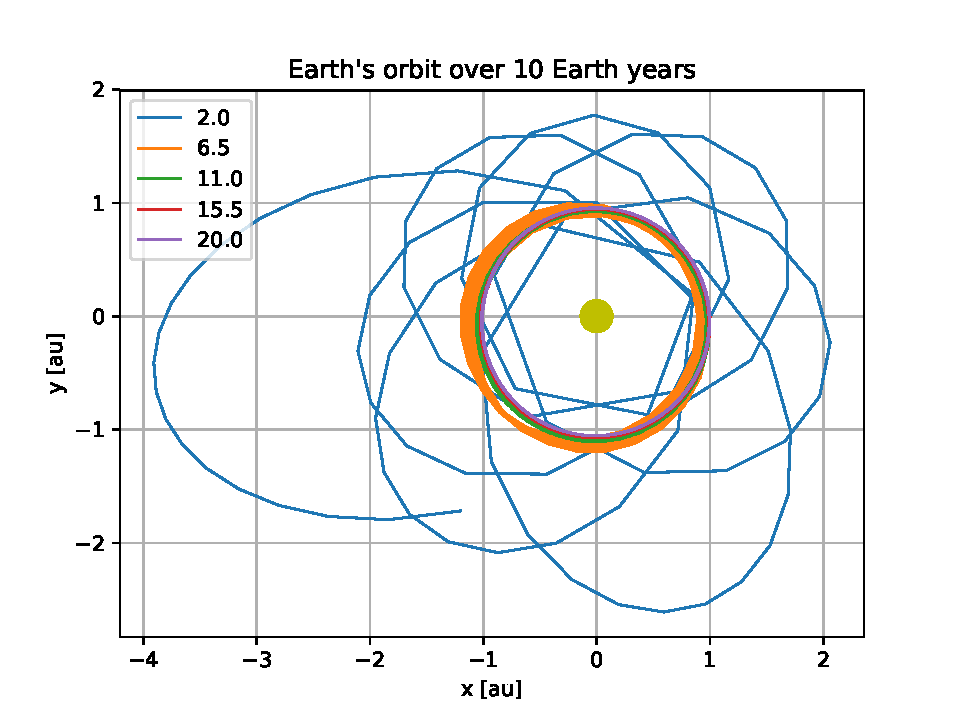
\includegraphics[width = 0.66\textwidth]{images/Earth_Trajectory_10.pdf}
                \caption{The trajectory of Earth over 10 Earth years for several different scaling parameters $\alpha$, and therefore different time steps.}
                \label{fig:Earth_trajectory}
            \end{figure}
            
            In figure (\ref{fig:rate_vs_length}) we can see that the rate of precession is on the scale of hundreds of arcseconds per century for a relatively short simulation time of around one Earth year.  The precession rate quickly decreases and seems to converge as the length of the simulation is increased past 20 Earth years.  We stop this test at a length of 100 Earth years because, in this simulation, the parameters used were that of the Sun-Mercury system, and the known value of Mercury's perihelion shift is about 43 arcseconds per century.
            
            \begin{figure}[t!]
                \centering
                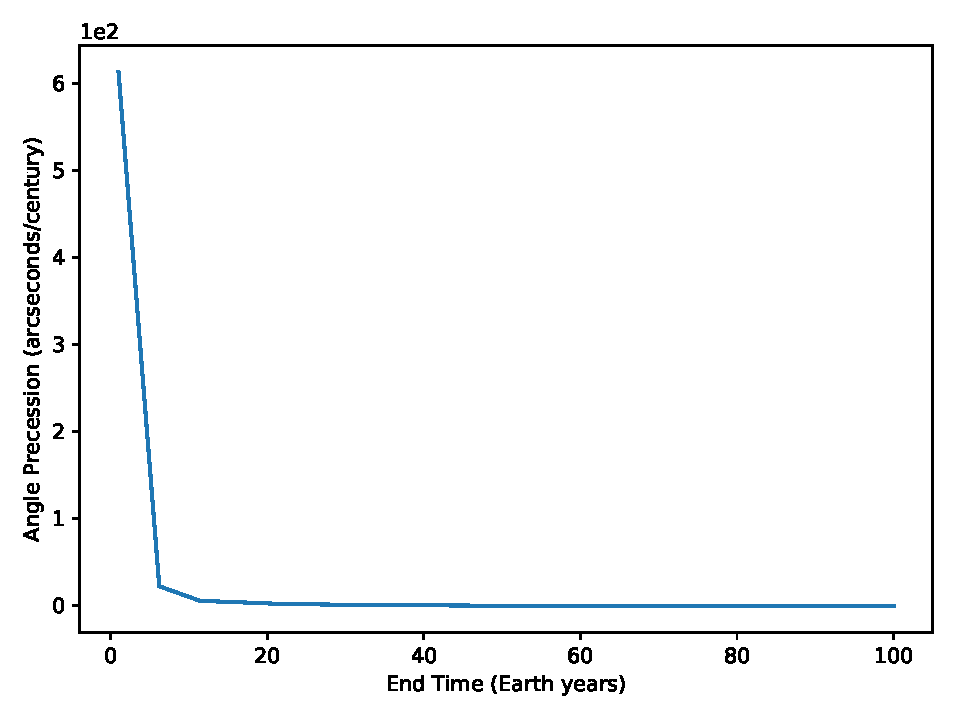
\includegraphics[width = 0.66\textwidth]{images/Precession_rate_Runtime_Comparison.pdf}
                \caption{The precession rate as a function of the length of the simulation.  The parameters used in this simulation were that of the Sun-Mercury system.}
                \label{fig:rate_vs_length}
            \end{figure}
            
            Now that we're (hopefully) at least somewhat confident the algorithm produces physically accurate results, let's analyze the Sun-Mercury system.

        \subsection{Results}

            \begin{figure}[h]
                \centering
                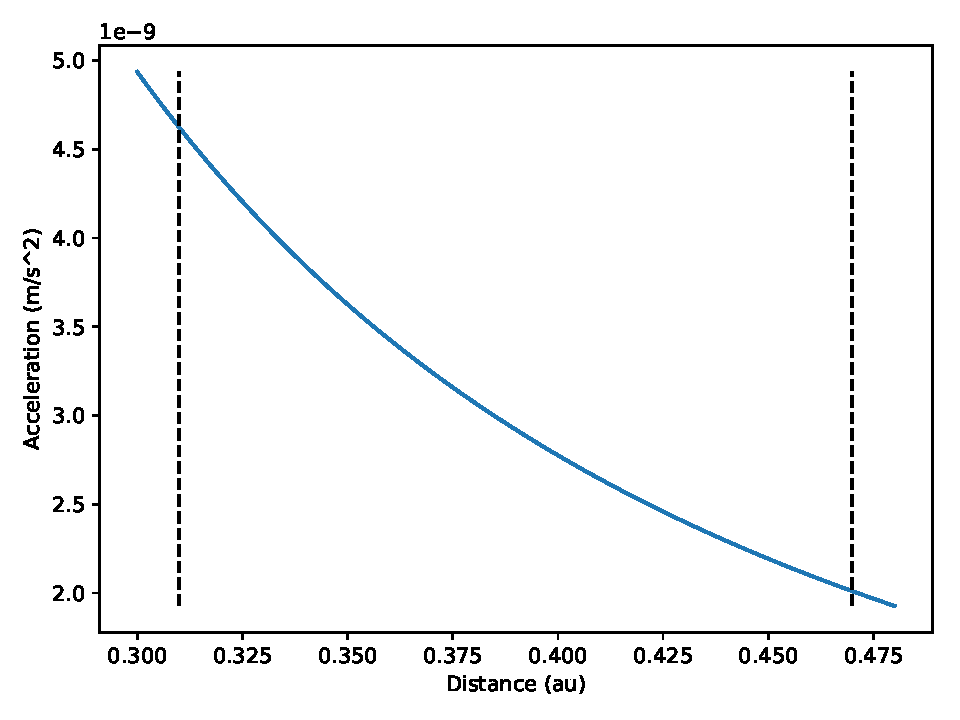
\includegraphics[width = 0.66\textwidth]{images/Newton_GR_Comp_Mercury.pdf}
                \caption{The strength of the gravitational acceleration from the Sun due to GR in the regime of Mercury's orbital distance.  The vertical dashed, black lines correspond to the distance between Mercury and the Sun at Mercury's perihelion and its aphelion.}
                \label{fig:GR_at_Mercury}
            \end{figure}
        
            Starting off, all the following results were done for the Sun-Mercury system, and with Mercury starting at it's perihelion (about 0.3 AU) on the x-axis with its velocity at that point, a time-step scaling parameter of $\alpha = 2000$, and a simulation time of 100 Earth years.  We start at perihelion because then we know that the velocity is orthogonal to the position, and it's a good starting point nonetheless.  Before we actually look at some results, let's see the actual strength of the GR effects at Mercury.  In figure (\ref{fig:GR_at_Mercury}), we can see the effects of GR are \emph{quite} minuscule, on the order of nanometers, compared to the closer regimes as shown in figure (\ref{fig:Newton_GR_Comp}).
            
            Since the effects of GR are so small at Mercury, the orbit should be almost negligibly close to the Newtonian orbit.  That is, we shouldn't be able to see any difference over any reasonable time scale.  In figure (\ref{fig:mercury_trajectory}), that's exactly what we see.
            
            Though if we take a closer look, specifically at the angle of the perihelion at each orbit, we can see GR's almost hidden effects.  In figure (\ref{fig:mercury_precession}), we can see that the perihelion actually oscillates in it's angle, while still having a trend to decrease linearly.  It's here that the importance of the (ridiculously) small time step (of scale factor $\alpha = 2000$) is needed.  If the time step were any bigger the angular precession would not be on the right scale as the known 43 arcseconds per century. 
            
            That being said, I also don't know why the angle jumps up and oscillates with such high amplitude.  The main takeaway here though is that the overall behavior of the perihelion is that it does linearly shift with time.  In this case the overall rate of precession is around the known value (in magnitude) of 43 arcseconds per century, but, getting back to the main idea, what how would this change with different eccentricity?
            
            In figures (\ref{fig:rate_vs_eccentricity}) and (\ref{fig:rate_vs_eccentricity_final}), we see how the rate of precession changes as the eccentricity of the orbit changes.  Well, the overall behavior is there.  As we increase eccentricity, the rate of precession decreases.
            
            In this analysis, only eccentricities $\epsilon < 0.8$ were considered because the implementation evolved the simulation in time, and since an increase in eccentricity corresponds to a non-linear increase in orbital period, the computation times associated with eccentricities $\epsilon > 0.8$ were unreasonably large.
            
            \begin{figure}[h]
                \centering
                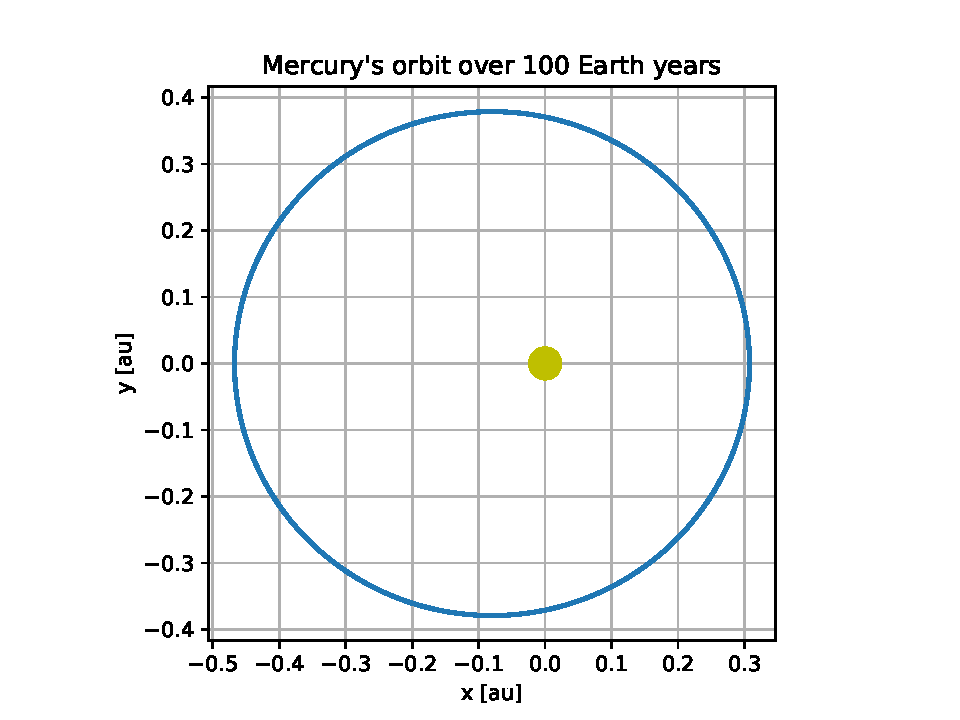
\includegraphics[width = 0.66\textwidth]{images/Trajectory_100.pdf}
                \caption{The trajectory of Mercury under the influence of MOND over the course of 100 Earth years.}
                \label{fig:mercury_trajectory}
            \end{figure} 
            
            \begin{figure}[h]
                \centering
                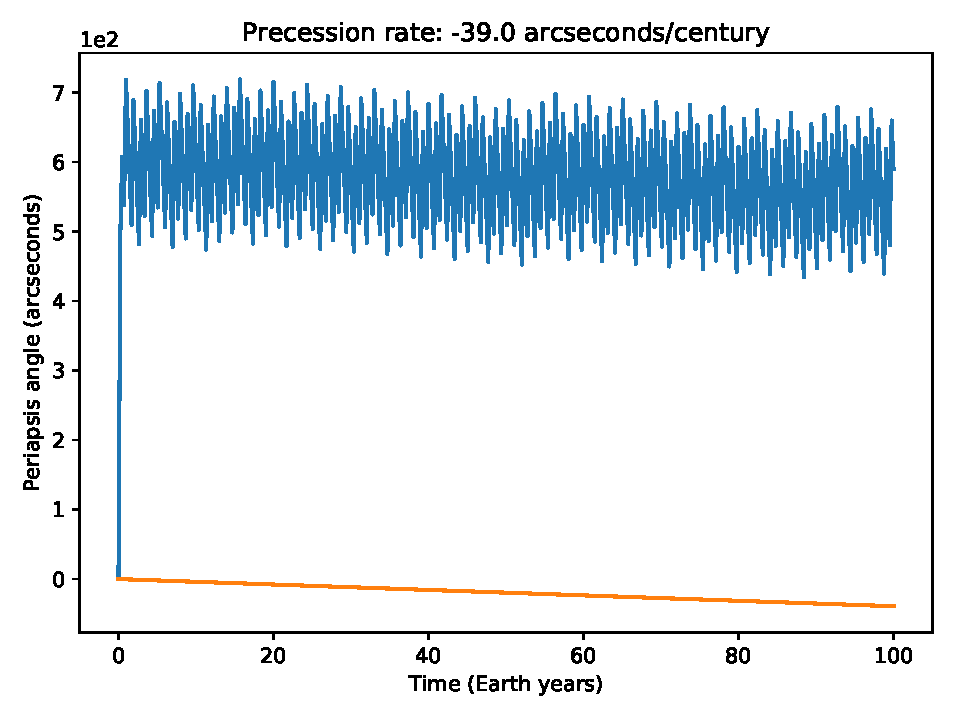
\includegraphics[width = 0.66\textwidth]{images/Precession_Angle_100.pdf}
                \caption{The angular precession of the perihelion of Mercury over the course of 100 Earth years.}
                \label{fig:mercury_precession}
            \end{figure}
            
            \begin{figure}[h]
                \centering
                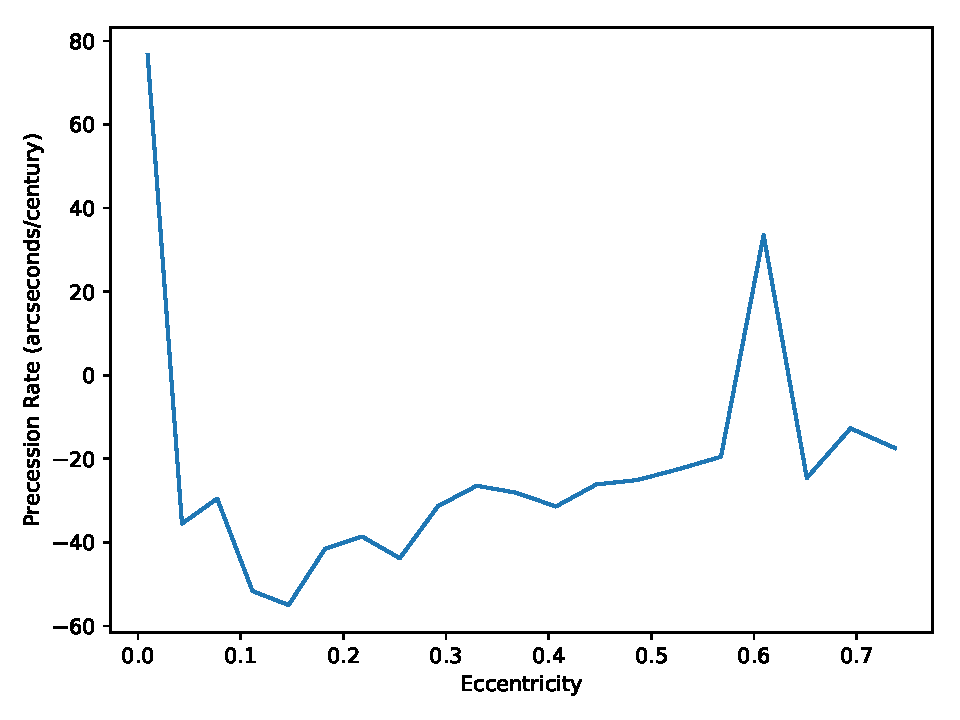
\includegraphics[width = 0.66\textwidth]{images/rate_v_eccentricity.pdf}
                \caption{The rate precession of Mercury if it had different eccentricities.}
                \label{fig:rate_vs_eccentricity}
            \end{figure}
            
            \begin{figure}[h]
                \centering
                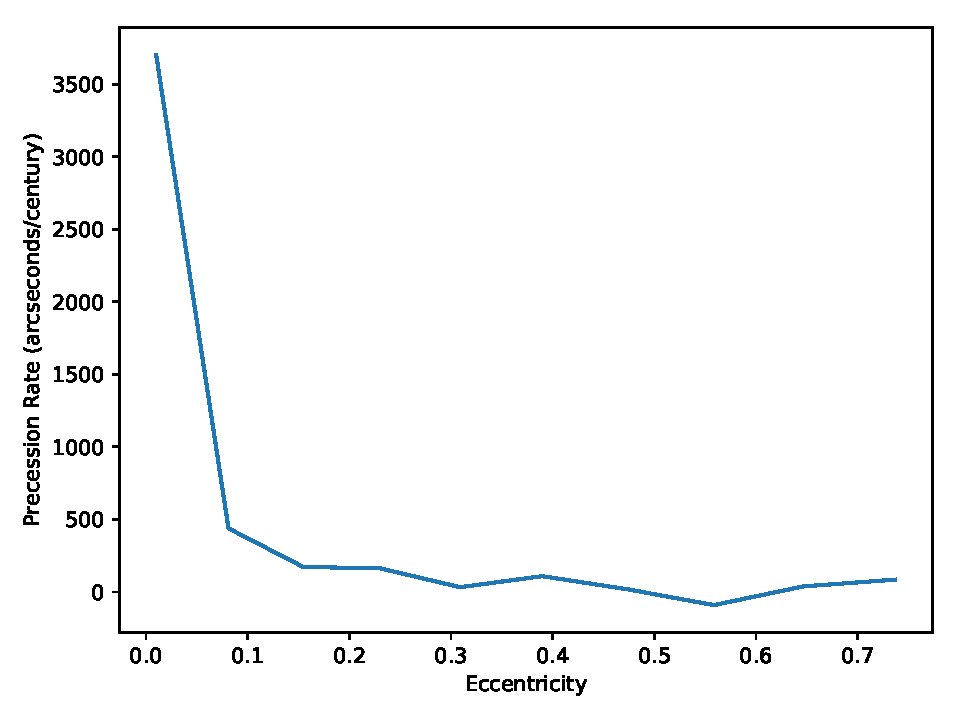
\includegraphics[width = 0.66\textwidth]{images/rate_v_eccentricity_final.pdf}
                \caption{The rate precession of Mercury if it had different eccentricities.  Each simulation here was done with a simulation time of 20 Earth years.}
                \label{fig:rate_vs_eccentricity_final}
            \end{figure}

\clearpage

    \section{Leading Order Gravitational Wave Frequencies from Short-Term Post-Newtonian Orbits via Fourth-Order Symplectic Integration}

        The following is work I completed for the final project in my graduate course ``Physics 561: Advanced Computational Physics''\cite{Chapman2022}.

        \subsection{Mathematical Model}

            % Weak field
            At its core, General Relativity (GR) is composed of 16 highly-coupled, nonlinear partial differential equations known as the Einstein Field Equations.  These equations are only able to be analytically solved without approximation for a few particularly symmetric physical systems\footnote{See the famous Schwarzchild solution.}.  The remaining systems require either to be approximated or solved numerically.  One type of system that actually falls in both categories is those where the gravitational effects are sufficiently weak.  These are called ``weak-field'' systems (WFS).  GR also predicts that all systems with a changing mass distribution (e.g. orbits) emit gravitational waves (GW), WFS by naturally emit low-amplitude gravitational waves.

            % Post-Newtonian
            While WFS can be approximated in several ways, we will further focus our attention on slightly changing Newtonian physics to account for only the strongest relativistic effects.  This is called a Post-Newtonian approximation (PNA).  PNA is also able to pick out the strongest part of the emitted low-amplitude gravitational waves.  The strongest part being the leading order frequency of the gravitational wave.

            % Numerically
            Even though weak-field systems are able to be solved analytically after being first-order approximated, the analytic methods are still quite complex and near unapproachable.  In this case, it would be easier (and for more complex systems, necessary) to solve and simulate the system with numerical methods.  When simulated, finding the properties of the system is just a matter of directly measuring them.

            With all of these in hand, the rest of this paper focuses on numerically simulating the dynamics of particles (such as Mercury) in WFS under a PNA in order to measure the leading order frequency of the emitted gravitational waves.

            \subsubsection{Inspiral \& Gravitational Waves}

                The most common way GW are produced is when a planet or star orbits around its parent star.  As these waves are emitted, they carry energy away from the system.  Then, due to conservation of momentum, the radius of the orbit shrinks and the speed of the object increases.  This increase in speed and proximity yields the emission of higher amplitude GW.  These higher amplitude GW carry even more energy away from the system, cause the orbit to shrink and speed up.  It is obvious these effects yield a positive feedback loop (Fig \ref{fig:GW_Loop}) that will only cease when the object collapses into its parent.  In the context of binary neutron star and black hole mergers, this moment is known as coalescence as they physically merge into a single body. 

                \begin{figure}[h]
                    \centering
                    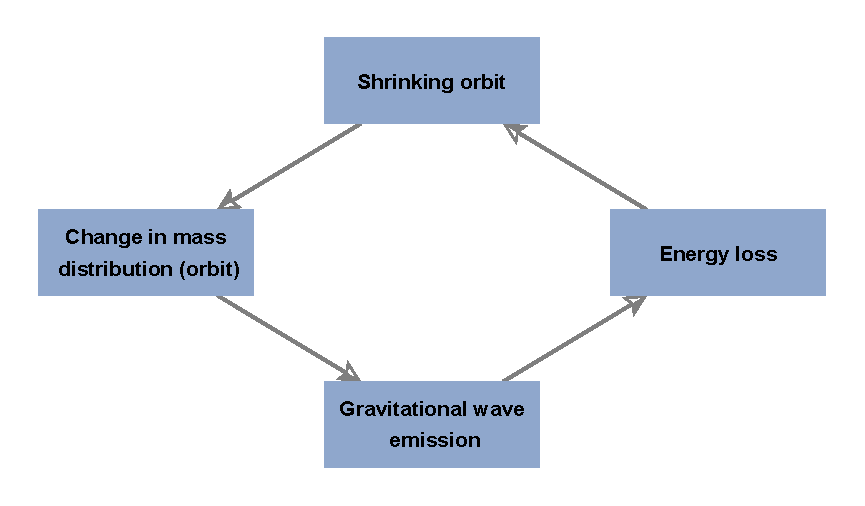
\includegraphics[width=0.66\textwidth]{images/GW_flow_diagram.pdf}
                    \caption{The emission of gravitational waves induces a feedback loop that causes more and more, stronger and stronger gravitational waves.}
                    \label{fig:GW_Loop}
                \end{figure}

            \subsubsection{Post-Newtonian Approximations}

                In this investigation, the PNA is implemented by incorporating a ``relativistic'' factor into Newtonian gravity (Eq. \ref{eq:PNA}) (in terms of the Schwarzchild radius of the parent body)\cite{Mercury_Euler}.

                \begin{align} \label{eq:PNA}
                    &\text{Newtonian} & &\text{Relativistic Correction} \nonumber \\
                    \ddot{\vec{r}} &= - \frac{c^2}{2} \frac{r_S}{r^2} \frac{\Vec{r}}{r} & \ddot{\vec{r}} &= - \frac{c^2}{2} \frac{r_S}{r^2} \underbrace{\left( 1 + 3 \frac{r_L^2}{r^2} \right)}_\text{Relativity} \frac{\Vec{r}}{r}
                \end{align}
                % Adiabatic
                Since PNA is only valid for WFS, the system cannot be modeled up to coalescence as the GW emitted at and relatively prior are well within the strong-field regime.  PNA does yield valid modelling until the time scale on which the orbital radius shrinks is comparable to the orbital period.  This point is called the adiabatic limit\cite{BaumgarteShapiro2021}.  Therefore, the investigations presented here will focus on the relatively early stages of the collapse.
                % GW Freq = 2P
                It is also the case that in WFS under a PNA, the leading order gravitational wave frequency is double the orbital frequency\cite{BaumgarteShapiro2021}.

        \subsection{Computational Model}

            For many-iteration gravitational simulations such as these, it is best to use an algorithm that has little error in energy conservation.  There is the class of numerical integrator called ``symplectic'' integrators that do just this.  There are a few different, easily-implementable, symplectic methods that could and have been used in the past for simulations such as those in this investigation. The first-order symplectic Euler-Cromer\cite{Mercury_Euler} method and the second-order symplectic Verlet\cite{Chapman_2019} methods have been used in the past to relative success but for much smaller time scales.

            Since the time scale on which the dynamics of a solar system significantly change is on the order of millions of years, it is also prudent to use an algorithm that is still substantially accurate for larger time steps.  The natural choice, given the previously used methods and time scales, is to increase the order of accuracy of the integrator.  Such methods seem to be novel, but both analytic and numeric work has been done to find them\cite{YOSHIDA1990262}.

            \begin{center} 
                $4 \mathcal{O}$ symplectic Yoshida integrator\cite{YOSHIDA1990262} 
            \end{center}
            \begin{align} \label{eq:Yoshida}
                x_i^0 &= x_i & x_i^n &= x_i^{n - 1} + c_n v_i^{n - 1} \Delta t & x_{i + 1} &= x_i^4 \\
                v_i^0 &= v_i & v_i^n &= v_i^{n - 1} + d_n \underbrace{a \left( x_i^n, v_i^{n - 1} \right)}_\text{``leapfrog''} \Delta t & v_{i + 1} &= v_i^4
            \end{align}

            The algorithm in Eq. (\ref{eq:Yoshida}) has been modified from its original presentation to have the acceleration include a dependence on the velocity.  The original algorithm only had acceleration dependent on position.

\pagebreak

        \subsection{Numerical Analysis}

            Previous work\cite{SymplecticNBody} has been done with similar integrators such as Wisdom-Holman in very similar systems.  The results of those investigations (Fig \ref{fig:Accuracy}) showed that integrators such as the fourth-order symplectic Yoshida, the error of the algorithm was and stayed sufficiently small for simulations within the time scale considered here.

            \begin{figure}[h]
                \centering
                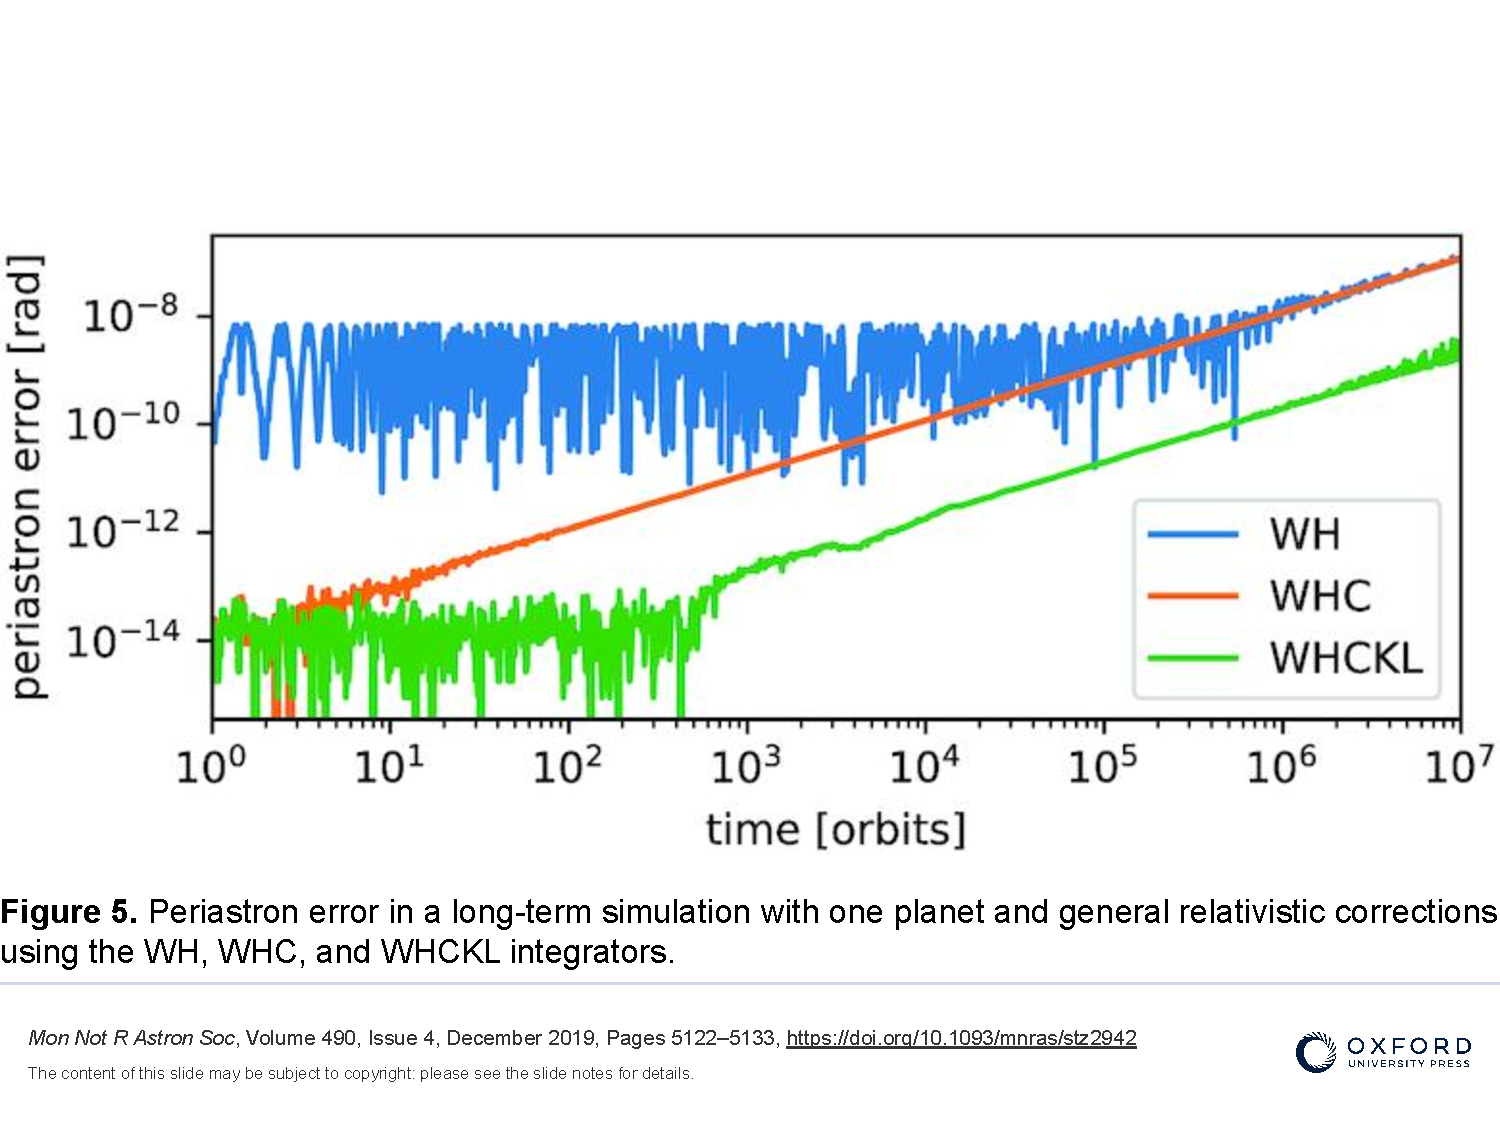
\includegraphics[width=0.66\textwidth]{images/Accuracy_plot.pdf}
                \caption{Significantly low error for symplectic integrators in a weakly relativistic system.}
                \label{fig:Accuracy}
            \end{figure}

% \pagebreak

        \subsection{Results}

            One of the most famous results for weak-field effects is the precession of Mercury's perihelion.  Over the course of $10^5$ Earth-years, this model shows (Fig: \ref{fig:Trajectory}) significant precession.  The angle of the perihelion with respect to the positive x-axis show is known to have a precession rate of about 43''/century.  So in order to validate the results we have from this investigation, we calculate the precession of measured periapsides.  Our results are inline with the observed value.  For each orbit, if the orbital period is measured, then the leading order of the emitted GW is twice that of the orbital period\cite{Mercury_Euler}.  Even for 100,000 years, there is insignificant change in the frequency of the emitted GW.

            \begin{figure}[h!]
                \centering
                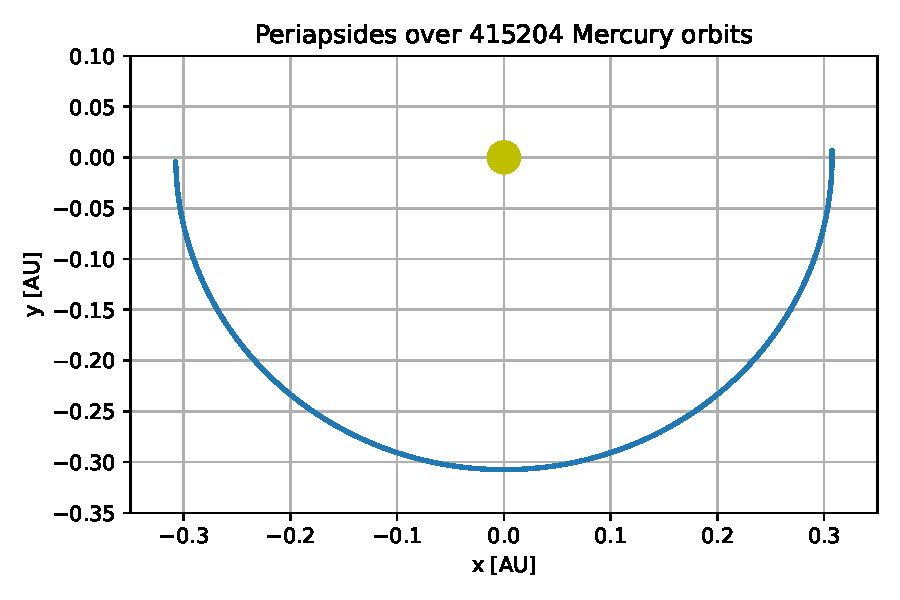
\includegraphics[width=0.66\textwidth]{images/Periapsis_Precession_100000.pdf}
                \caption{Precession of Mercury's perihelion}
                \label{fig:Trajectory}
            \end{figure}
        
            \begin{figure}[h]
                \centering
                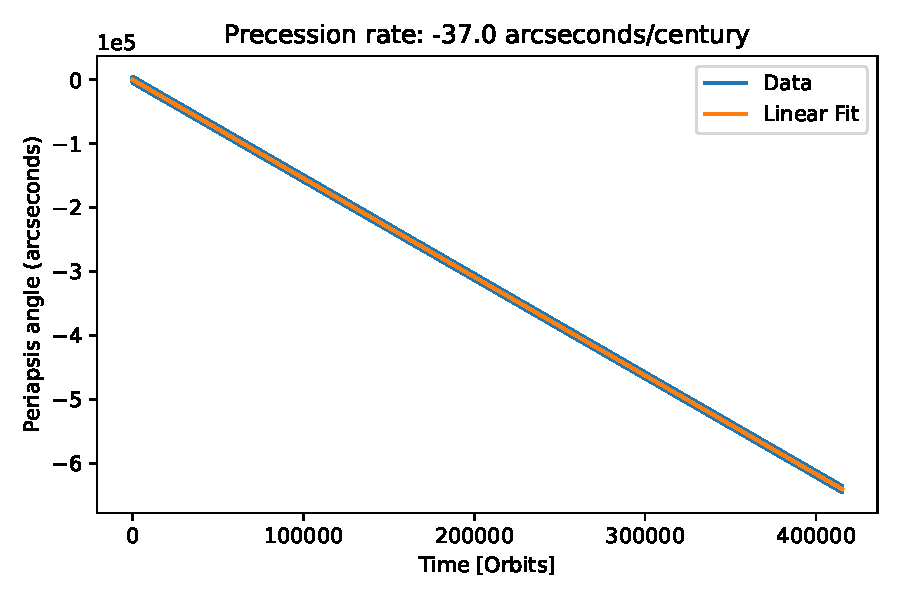
\includegraphics[width=0.66\textwidth]{images/Periapsis_angle_legended100000.pdf}
                \caption{Linear change in Mercury's perihelion angle.}
                \label{fig:Angle}
            \end{figure}
        
            \begin{figure}
                \centering
                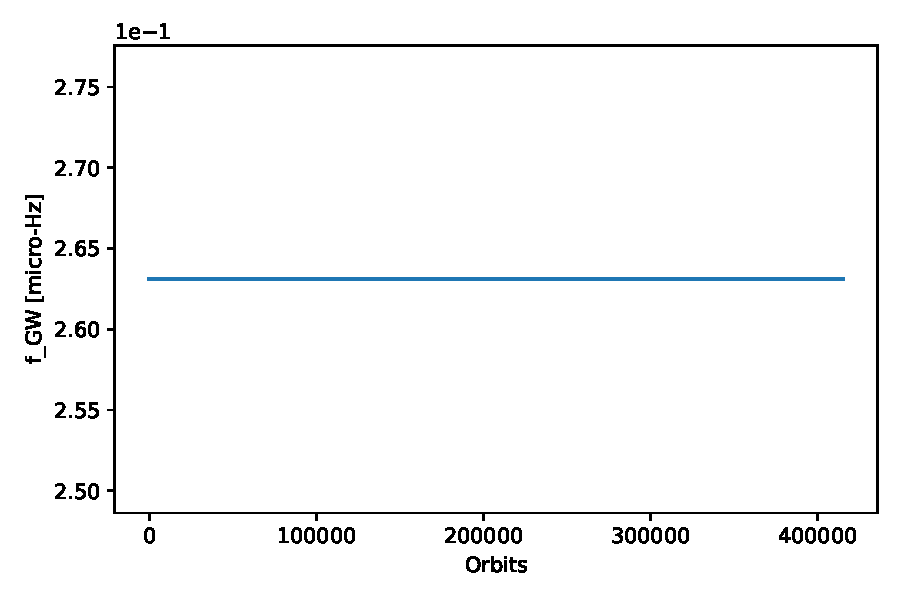
\includegraphics[width=0.66\textwidth]{images/GW_freq_100000.pdf}
                \caption{Leading order frequency Mercury's GW}
                \label{fig:GWFreq}
            \end{figure}

        \subsection{Discussion}

            These results show that a WFS under PNA evolved with a fourth-order symplectic integrator yields simulated properties that are inline with experimental observation.  These results also show the time scale on which the dynamics of the solar system significantly change is even much longer than 100,000 years.

        \subsection{Conclusion}

            Overall, analytic descriptions of general relativistic systems is near impossible for any moderately real system.  Because of this, numerical is often preferred if not needed.  Such simulations are even more implementable if they are approached by simply augmenting Newtonian physics for weak-field systems.  These approaches are yield relatively accurate results, both in error and in agreement with observation, if implemented with a high-order symplectic integrator.

\chapter{Conclusion}

    Computational physics covers all domains of physics and science.  Because real world problems are so much more complex than theory can manipulate, numerical methods are needed in order to make realistic predictions.  Many of these numerical implementations require the use of high-performance methods.  Computaitonal physics is a vast field with many many opportunities in which to apply both a deep understanding of physics, math, and computer science.

\pagebreak
\printbibliography

\printindex

\end{document}